%% 
%% Copyright 2007-2020 Elsevier Ltd
%% 
%% This file is part of the 'Elsarticle Bundle'.
%% ---------------------------------------------
%% 
%% It may be distributed under the conditions of the LaTeX Project Public
%% License, either version 1.2 of this license or (at your option) any
%% later version.  The latest version of this license is in
%%    http://www.latex-project.org/lppl.txt
%% and version 1.2 or later is part of all distributions of LaTeX
%% version 1999/12/01 or later.
%% 
%% The list of all files belonging to the 'Elsarticle Bundle' is
%% given in the file `manifest.txt'.
%% 
%% Template article for Elsevier's document class `elsarticle'
%% with Harvard style bibliographic references

%\documentclass[preprint,12pt,authoryear]{elsarticle}
%\documentclass[3p, 12pt,authoryear]{elsarticle}
\documentclass[final, 3p, times, authoryear]{elsarticle}

%% Use the option review to obtain double line spacing
%% \documentclass[authoryear,preprint,review,12pt]{elsarticle}

%% Use the options 1p,twocolumn; 3p; 3p,twocolumn; 5p; or 5p,twocolumn
%% for a journal layout:
%% \documentclass[final,1p,times,authoryear]{elsarticle}
%% \documentclass[final,1p,times,twocolumn,authoryear]{elsarticle}
%% \documentclass[final,3p,times,authoryear]{elsarticle}
%% \documentclass[final,3p,times,twocolumn,authoryear]{elsarticle}
%% \documentclass[final,5p,times,authoryear]{elsarticle}
%% \documentclass[final,5p,times,twocolumn,authoryear]{elsarticle}

%% For including figures, graphicx.sty has been loaded in
%% elsarticle.cls. If you prefer to use the old commands
%% please give \usepackage{epsfig}

%% The amssymb package provides various useful mathematical symbols
\usepackage{amssymb}
%% The amsthm package provides extended theorem environments
\usepackage{amsmath,amsthm}

%% The lineno packages adds line numbers. Start line numbering with
%% \begin{linenumbers}, end it with \end{linenumbers}. Or switch it on
%% for the whole article with \linenumbers.
%% \usepackage{lineno}

\usepackage{hyperref}
%\usepackage{tikz}
%\usetikzlibrary{mindmap}
\usepackage{multirow}
\usepackage{pgfplots}
\usepackage{arydshln}
\usepackage{paralist}
\usepackage{booktabs}

%% Comments
\newif\ifcomments\commentstrue

\ifcomments
\newcommand{\authornote}[3]{\textcolor{#1}{[#3 ---#2]}}
\newcommand{\todo}[1]{\textcolor{red}{[TODO: #1]}}
\else
\newcommand{\authornote}[3]{}
\newcommand{\todo}[1]{}
\fi

\newcommand{\wss}[1]{\authornote{blue}{SS}{#1}} %Spencer Smith
\newcommand{\jc}[1]{\authornote{red}{JC}{#1}} %Jacques Carette
\newcommand{\mn}[1]{\authornote{magenta}{MN}{#1}} %Mike Noseworthy
\newcommand{\ad}[1]{\authornote{cyan}{AD}{#1}} %Ao Dong

\newcommand{\notdone}[1]{\textcolor{red}{#1}}
\newcommand{\done}[1]{\textcolor{black}{#1}}

\newcounter{rqnum} %research question number
\newcommand{\rqtherqnum}{RQ`'\therqnum}
\newcommand{\rqref}[1]{RQ\ref{#1}}

\newcounter{pnum} %pain point number
\newcommand{\ppthepnum}{P`'\thepnum}
\newcommand{\ppref}[1]{P\ref{#1}}

\journal{Academic Radiology}

%\pgfplotsset{compat=1.13}

\begin{document}

\begin{frontmatter}

%% Title, authors and addresses

%% use the tnoteref command within \title for footnotes;
%% use the tnotetext command for theassociated footnote;
%% use the fnref command within \author or \affiliation for footnotes;
%% use the fntext command for theassociated footnote;
%% use the corref command within \author for corresponding author footnotes;
%% use the cortext command for theassociated footnote;
%% use the ead command for the email address,
%% and the form \ead[url] for the home page:
%% \title{Title\tnoteref{label1}}
%% \tnotetext[label1]{}
%% \author{Name\corref{cor1}\fnref{label2}}
%% \ead{email address}
%% \ead[url]{home page}
%% \fntext[label2]{}
%% \cortext[cor1]{}
%% \affiliation{organization={},
%%            addressline={}, 
%%            city={},
%%            postcode={}, 
%%            state={},
%%            country={}}
%% \fntext[label3]{}

\title{State of the Practice for Medical Imaging Software}

%% use optional labels to link authors explicitly to addresses:
%% \author[label1,label2]{}
%% \affiliation[label1]{organization={},
%%             addressline={},
%%             city={},
%%             postcode={},
%%             state={},
%%             country={}}
%%
%% \affiliation[label2]{organization={},
%%             addressline={},
%%             city={},
%%             postcode={},
%%             state={},
%%             country={}}

\author[CAS]{Spencer Smith}
\author[CAS]{Ao Dong}
\author[CAS]{Jacques Carette}
\author[ECE]{Mike Noseworthy}

\affiliation[CAS]{organization={McMaster University, Computing and Software Department},%Department and Organization
            addressline={1280 Main Street West}, 
            city={Hamilton},
            postcode={L8S 4K1}, 
            state={Ontario},
            country={Canada}}

\affiliation[ECE]{organization={McMaster University, Electrical Engineering},%Department and Organization
            addressline={1280 Main Street West}, 
            city={Hamilton},
            postcode={L8S 4K1}, 
            state={Ontario},
            country={Canada}}

\begin{abstract}

We present the state of the practice for Medical Imaging software. We selected
29 medical imaging projects from 48 candidates, assessed 10 software qualities
(installability, correctness/ verifiability, reliability, robustness, usability,
maintainability, reusability, understandability, visibility/transparency and
reproducibility) by answering 108 questions for each software project, and
interviewed 8 of the 29 development teams. Based on the quantitative data for
the first 9 qualities, we ranked the MI software with the Analytic Hierarchy
Process (AHP). The top three software products were \textit{3D Slicer},
\textit{ImageJ}, and \textit{OHIF Viewer}. By interviewing the developers, we
identified three major pain points: i) lack of resources; ii) difficulty
balancing between compatibility, maintainability, performance, and security;
and, iii) lack of access to real-world datasets for testing. For future MI
software projects, we propose adopting test-driven development, using continuous
integration and continuous delivery (CI/CD), using git and GitHub, maintaining
good documentation, supporting third-party plugins or extensions, considering
web application solutions, and improving collaboration between different MI
software projects. \wss{Update after the paper has been revised.}

\end{abstract}

%%Graphical abstract
%\begin{graphicalabstract}
%\includegraphics{grabs}
%\end{graphicalabstract}

%%Research highlights
%\begin{highlights}
%\item Research highlight 1
%\item Research highlight 2
%\end{highlights}

\begin{keyword}
	medical imaging, research software, software engineering, software
	quality, Analytic Hierarchy Process, developer interviews
\end{keyword}

\end{frontmatter}

%% \linenumbers

\section{Introduction} \label{ch_intro}

We aim to study the state of software development practice for Medical Imaging
(MI) software.  MI tools use images of the interior of the body (from sources
such as Magnetic Resonance Imaging (MRI), Computed Tomography (CT), Positron
Emission Tomography (PET) and Ultrasound) to provide information for diagnostic,
analytic, and medical applications \citep{FDA2021, enwiki:1034887445,
Zhang2008}.  An example medical image of the brain is provided in
Figure~\ref{Fig_Example}. Given the importance of MI software and the high
number of competing software projects, we wish to understand the merits and
drawbacks of the current development processes, tools and methodologies.  We aim
to assess through a software engineering lens the quality of the existing
software with the hope of highlighting standout examples, understanding current
pain points and providing guidelines and recommendations for future development.

\begin{figure}[!ht]
    \begin{center}
        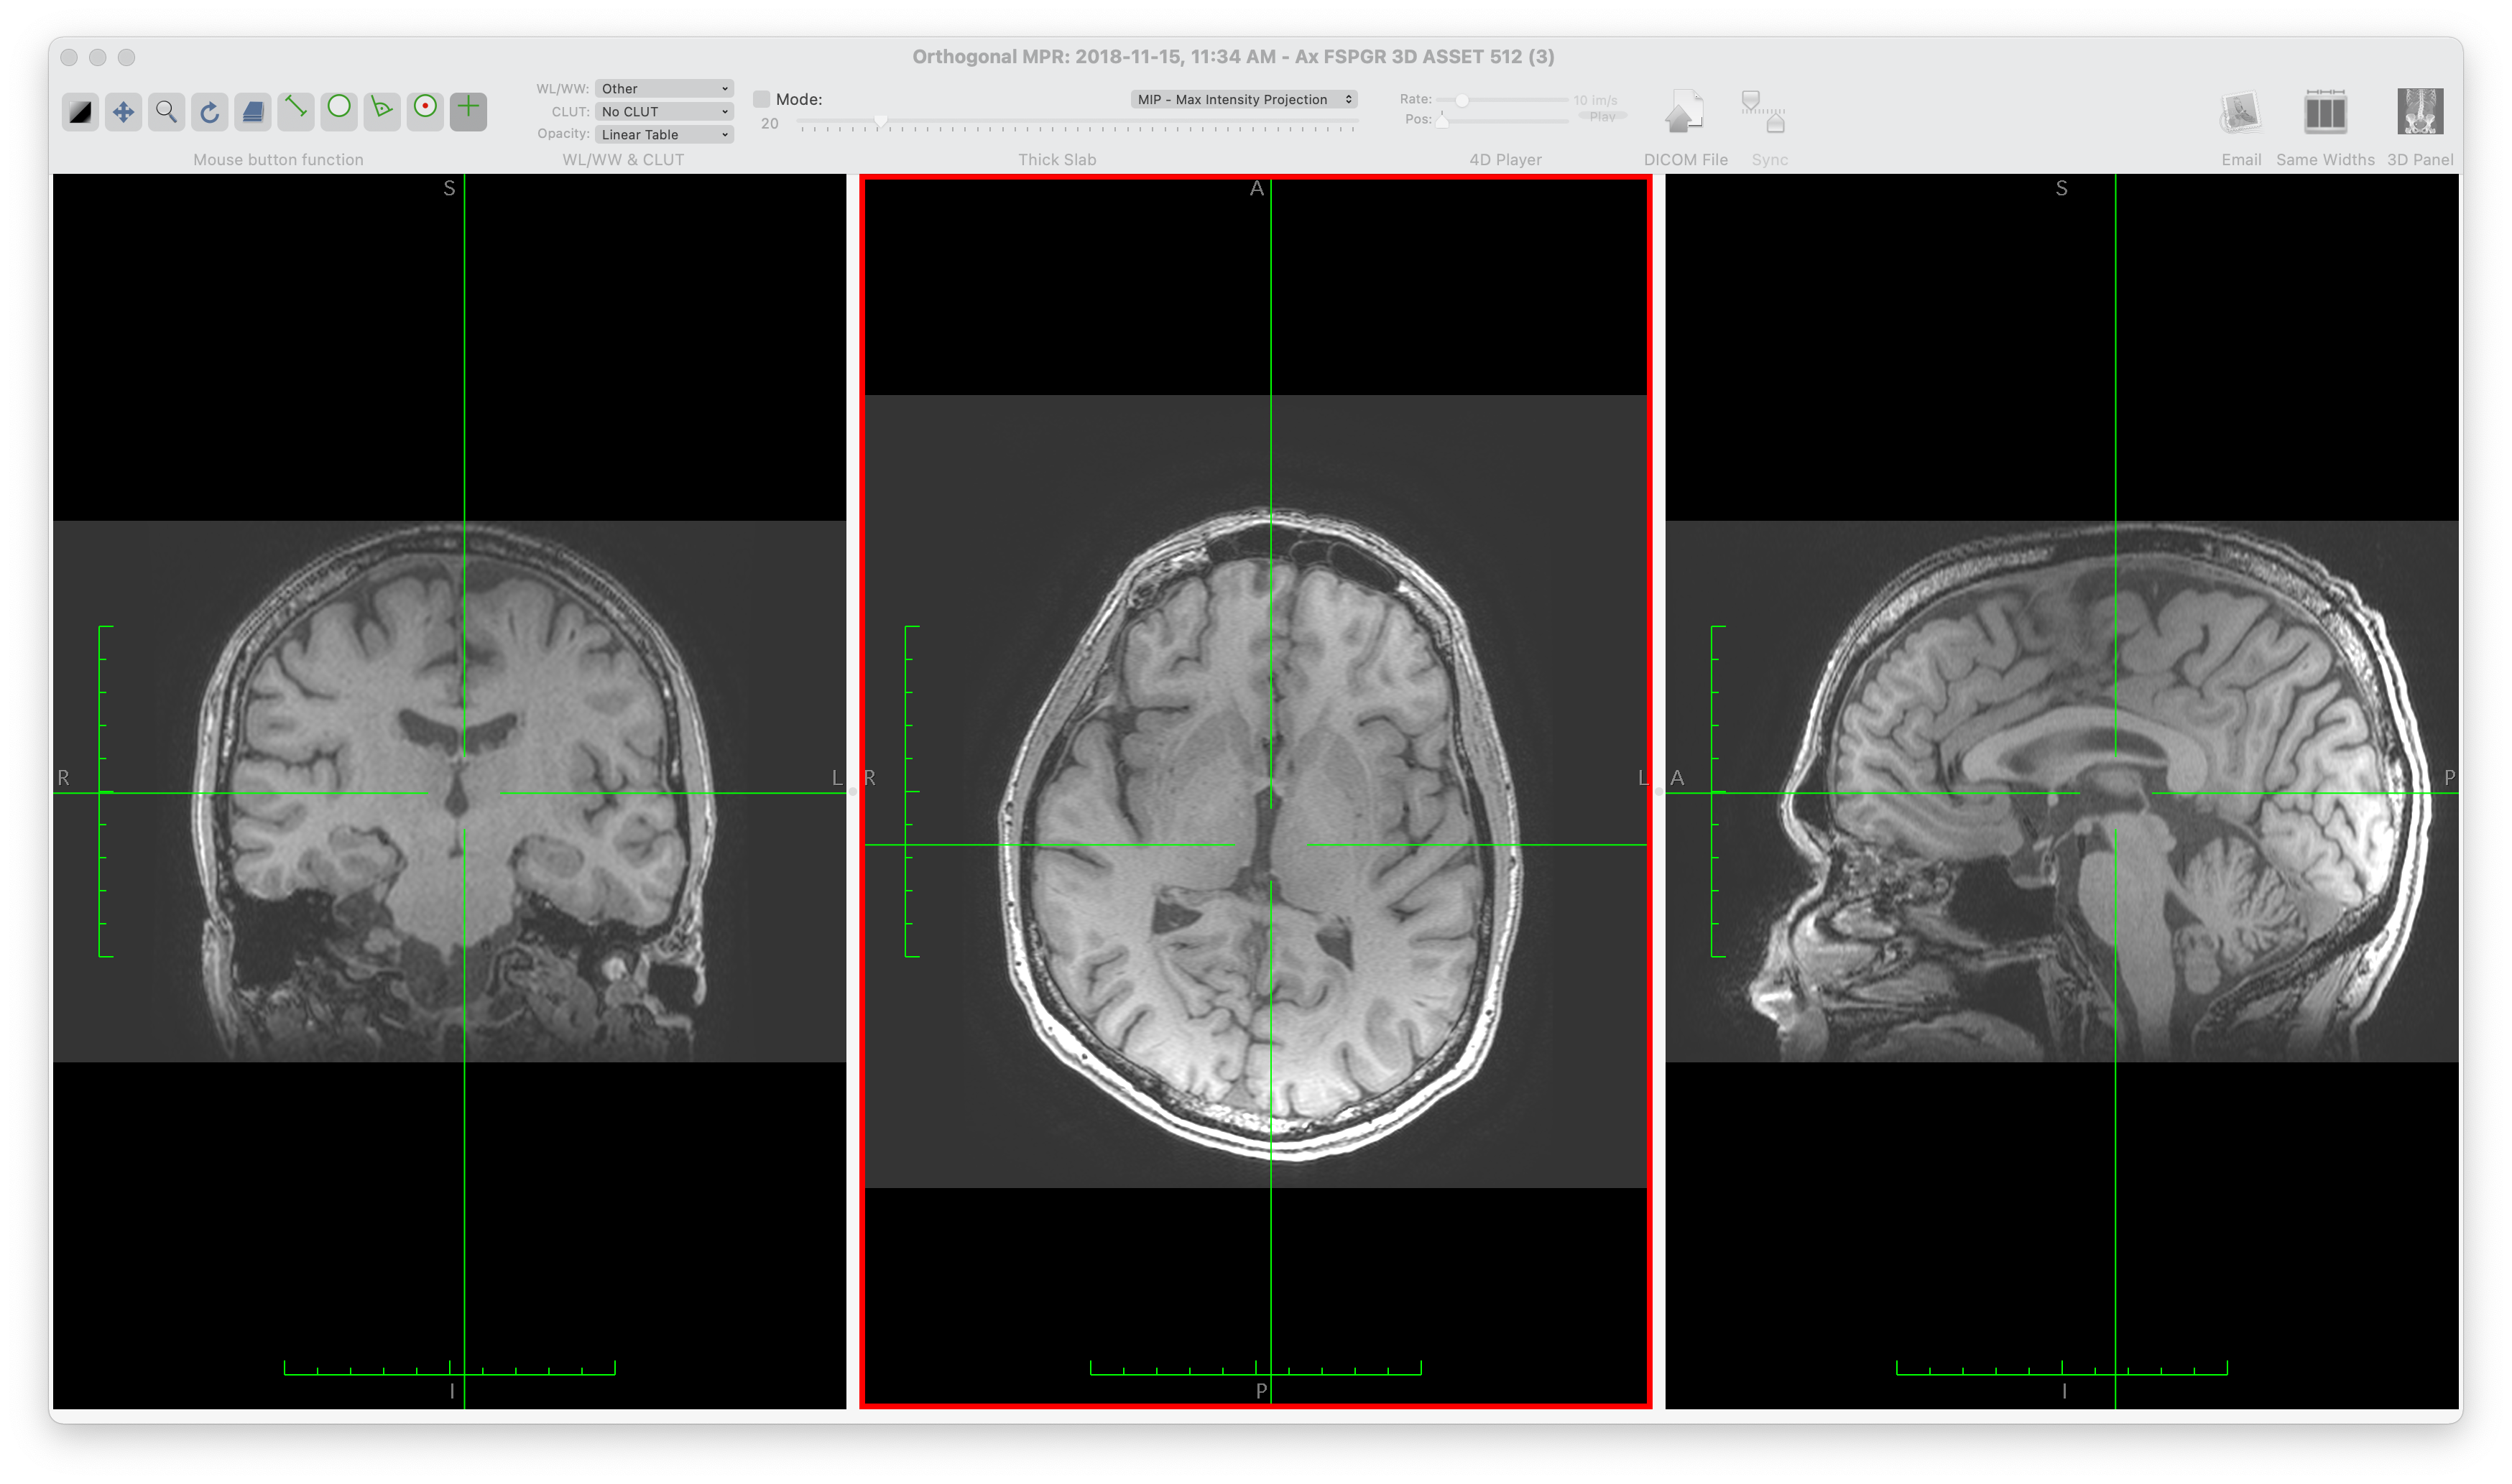
\includegraphics[scale=0.25]{figures/MPR.png}        
    \end{center}
    \caption{Example brain image showing a multi-planar reformat using Horos (free open-source medical imaging/DICOM viewer for OSX, based on OsiriX)}
    \label{Fig_Example}
\end{figure}
    
\subsection{Research Questions} \label{sec_motivation}

Not only do we wish to gain insight into the state of the practice for MI
software, we also wish to understand the development of research software in
general. We wish to understand the impact of the often cited gap, or chasm,
between software engineering and scientific programming \citep{Kelly2007,
Storer2017}. Although scientists spend a substantial proportion of their working
hours on software development \citep{Hannay2009, Prabhu2011}, many developers
learn software engineering skills by themselves or from their peers, instead of
from proper training \citep{Hannay2009}. \citet{Hannay2009} observe that many
scientists showed ignorance and indifference to standard software engineering
concepts. For instance, according to a survey by \citet{Prabhu2011}, more than
half of their 114 subjects did not use a proper debugger when coding.

To gain insights, we devised 10 research questions, which can be applied to MI,
as well as to other domains, of research software \citep{SmithEtAl2021}.  The
questions are designed to learn about the community's interest in, and
experience with, artifacts, tools, principles, processes, methodologies and
qualities.  When we mention artifacts we mean the documents, scripts and code
that constitutes a software development project. Example artifacts include
requirements, specifications, user manuals, unit tests, system tests, usability
tests, build scripts, API (Application Programming Interface) documentation,
READMEs, license documents, process documents, and code.  Once we have learned
what MI developers do, we then put this information in context by contrasting MI
software against the trends shown by developers in other research software
communities.  Our aim is to collect enough information to understand the current
pain points experienced by the MI software development community so that we can
make some preliminary recommendations for future improvements. 

The questions are used to structure the discussion in the paper, so for each
research question below we point to the section that contains our answer.  We
start with identifying the relevant examples of MI software:

\begin{enumerate}
	\item[RQ\refstepcounter{rqnum}\therqnum \label{RQ_WhatProjects}:] What MI
	software projects exist, with the constraint that the source code must be
	available for all identified projects? (Section~\ref{ch_results})
	\item [RQ\refstepcounter{rqnum}\therqnum \label{RQ_HighestQuality}:] Which
	of the projects identified in \rqref{RQ_WhatProjects} follow current best
	practices, based on evidence found by experimenting with the software and
	searching the artifacts available in each project's repository?
	(Section~\ref{ch_results})
	\item [RQ\refstepcounter{rqnum}\therqnum \label{RQ_CompareHQ2Popular}:] How
	similar is the list of top projects identified in \rqref{RQ_HighestQuality}
	to the most popular projects, as viewed by the scientific community?
	(Section~\ref{Sec_VsCommunityRanking})
    \item [RQ\refstepcounter{rqnum}\therqnum \label{RQ_CompareArtifacts}:] How
	do MI projects compare to research software in general with respect to the
	artifacts present in their repositories?
	(Section~\ref{Sec_CompareArtifacts})
	\item [RQ\refstepcounter{rqnum}\therqnum \label{RQ_CompareToolsProjMngmnt}:]
	How do MI projects compare to research software in general with respect to
	the use of tools (Section~\ref{Sec_CompareTools}) for:
	\begin{enumerate} 
		\item [\rqref{RQ_CompareToolsProjMngmnt}.a] development; and,
		\item [\rqref{RQ_CompareToolsProjMngmnt}.b] project management?
	\end{enumerate}
	\item [RQ\refstepcounter{rqnum}\therqnum \label{RQ_CompareMethodologies}:]
	How do MI projects compare to research software in general with respect to
	principles, processes and methodologies used?
	(Section~\ref{Sec_CompareMethodologies})
	\item [RQ\refstepcounter{rqnum}\therqnum \label{RQ_PainPoints}:] What are
	the pain points for developers working on MI software projects?
	(Section~\ref{painpoints})
	\item [RQ\refstepcounter{rqnum}\therqnum \label{RQ_ComparePainPoints}:] How
	do the pain points of developers from MI compare to the pain points
	for research software in general? (Section~\ref{painpoints})
	\item [RQ\refstepcounter{rqnum}\therqnum \label{RQ_Concerns}:] For MI
	developers what specific best practices are taken to address the pain points
	and software quality concerns? (Section~\ref{Sec_AddressConcerns})
	\item [RQ\refstepcounter{rqnum}\therqnum \label{RQ_Recommend}:]
	What research software development practice could potentially address the
	pain point concerns identified in \rqref{RQ_PainPoints}).
	(Section~\ref{ch_recommendations})

\end{enumerate}

\subsection{Scope} \label{sec_scope}

To make the project feasible, we only cover MI visualization software.  As a
consequence we are excluding many other categories of MI software, including
Segmentation, Registration, Visualization, Enhancement, Quantification,
Simulation, plus MI archiving and telemedicine systems (Compression, Storage,
and Communication) (as summarized by \citet{Bankman2000} and
\citet{Angenent2006}).  We also exclude Statistical Analysis and Image-based
Physiological Modelling \citep{enwiki:1034877594} and Feature Extraction,
Classification, and Interpretation \citep{Kim2011}. Software that provides MI
support functions is also out of scope; therefore, we have not assessed the
toolkit libraries VTK \citep{SchroederEtAl2006} and ITK \citep{McCormick2014}.
Finally, Picture Archiving and Communication System (PACS), which helps users to
economically store and conveniently access images \citep{Choplin1992}, are
considered out of scope. 

\subsection{Methodology Overview}

We designed a general methodology to assess the state of the practice for SC
software \citep{SmithEtAl2021}. Details can be found in
Section~\ref{ch_methods}.  Our methodology has been applied to MI software
\citep{Dong2021} and Lattice Boltzmann Solvers \citep{Michalski2021}.  This
methodology builds off prior work to assess the state of the practice for such
domains as Geographic Information Systems \citep{smith2018state}, Mesh
Generators \citep{smith2016state}, Seismology software
\citep{Smith2018Seismology}, and Statistical software for psychology
\citep{smith2018statistical}.  In keeping with the previous methodology, we have
maintained the constraint that the work load for measuring a given domain should
be feasible for a team as small as one person, and for a short time, ideally
around a person month of effort. A person month is considered to be $20$ working
days ($4$ weeks in a month, with $5$ days of work per week) at $8$ person hours
per day, or $20 \times 8 = 160$ person hours.

With our methodology, we first choose an SC domain (in the current case MI) and
identify a list of about 30 software packages. (For measuring MI we used 29
software packages.)  We approximately measure the qualities of each package by
filling in a grading template. Compared with our previous methodology, the new
methodology also includes repository based metrics, such as the number of files,
number of lines of code, percentage of issues that are closed, etc.  With the
quantitative data in the grading template, we rank the software with the
Analytic Hierarchy Process (AHP) (Details are found in
Section~\ref{ch_background}). After this, as another addition to our previous
methodology, we interview some of the development teams to further understand
the status of their development process.

\section{Background} \label{ch_background}

To measure the existing MI software we need two sets of definitions: i) the
definitions of relevant software license models (Section
\ref{sec_software_categories}); and, ii) the definitions of the software
qualities that we will be assessing (Section \ref{sec_software_quality}). In our
assessment we rank the software packages for each quality; therefore, this
section also provides the background on our ranking process -- the Analytic
Hierarchy Process (Section \ref{sec_AHP}).

\subsection{Software Categories} \label{sec_software_categories}

When assessing software packages, we need to know what license the software is
distributed under.  In particular, we need to know whether the source code will
be available to us or not.  We define three common software categories.  We will
only assess software that fits under the Open Source Software license.

\begin{itemize}

\item \textbf{Open Source Software (OSS)} For OSS, the source code is openly
accessible. Users have the right to study, change and distribute it under a
license granted by the copyright holder. For many OSS projects, the development
process relies on the collaboration of different contributors worldwide
\citep{Corbly2014}. Accessible source code usually exposes more ``secrets'' of a
software project, such as the underlying logic of software functions, how
developers achieve their works, and the flaws and potential risks in the final
product. Thus, it brings much more convenience to researchers analyzing the
qualities of the project.

\item \textbf{Freeware} Freeware is software that can be used free of charge.
Unlike OSS, the authors of do not allow access or modify the source code
\citep{LINFO2006}. To many end-users, the differences between freeware and OSS
may not be relevant. However, software developers who wish to modify the source
code, and researchers looking for insight into software development process may
find the inaccessible source code a problem. 

\item \textbf{Commercial Software} ``Commercial software is software developed
by a business as part of its business'' \citep{GNU2019}. Typically speaking, the
users are required to pay to access all of the features of commercial software,
excluding access to the source code. However, some commercial software is also
free of charge \citep{GNU2019}. Based on our experience, most commercial
software products are not OSS.

\end{itemize}

\subsection{Software Quality Definitions} \label{sec_software_quality}

Quality is defined as a measure of the excellence or worth of an entity.  As is
common practice, we do not think of quality as a single measure, but rather as a
set of measures.  That is, quality is a collection of different qualities, often
called ``ilities.''  Below we list the 10 qualities of interest for this study.
The order of the qualities follows the order used in \citet{GhezziEtAl2003},
which puts related qualities (like correctness and reliability) together.
Moreover, the order is roughly the same as the order qualities are considered in
practice.

\begin{itemize}
	\item \textbf{Installability} The effort required for the installation
    and/or uninstallation of software in a specified environment
    \citep{ISO/IEC25010, lenhard2013measuring}.

	\item \textbf{Correctness \& Verifiability} A program is correct if it
    matches its specification \citep[p.\ 17]{GhezziEtAl2003}.  The specification
    can either be explicitly or implicitly stated.  The related quality of
    verifiability is the ease with which the software components or the
    integrated product can be checked to demonstrate its correctness. 

	\item \textbf{Reliability} The probability of failure-free operation of a
	computer program in a specified environment for a specified time \citep{musa1987software}, \citep[p.\ 357]{GhezziEtAl2003}.

	\item \textbf{Robustness} Software possesses the characteristic of
	robustness if it behaves ``reasonably'' in two situations: i) when it
	encounters circumstances not anticipated in the requirements specification,
	and ii) when the assumptions in its requirements specification are violated
	\citep[p.\ 19]{GhezziEtAl2003}, \citep{boehm2007software}.

	\item \textbf{Usability} ``The extent to which a product can be used by
	specified users to achieve specified goals with effectiveness, efficiency,
	and satisfaction in a specified context of use'' \citep{ISO/TR16982:2002}
	\citep{ISO9241-11:2018}.

	\item \textbf{Maintainability} The effort with which a software system or
	component can be modified to i) correct faults; ii) improve performance or
	other attributes; iii) satisfy new requirements
	\citep{IEEEStdGlossarySET1990}, \citep{boehm2007software}.

	\item \textbf{Reusability} ``The extent to which a software component can be
	used with or without adaptation in a problem solution other than the one for
	which it was originally developed'' \citep{kalagiakos2003non}.

	\item \textbf{Understandability} ``The capability of the software product to
	enable the user to understand whether the software is suitable, and how it
	can be used for particular tasks and conditions of use'' \citep{iso2001iec}.

	\item \textbf{Visibility/Transparency} The extent to which all of the steps
	of a software development process and the current status of it are conveyed
	clearly \citep[p.\ 32]{GhezziEtAl2003}.

	\item \textbf{Reproducibility} ``A result is said to be reproducible if
	another researcher can take the original code and input data, execute it,
	and re-obtain the same result'' \citep{BenureauAndRougier2017}.
\end{itemize}

\subsection{Analytic Hierarchy Process (AHP)} \label{sec_AHP}

Thomas L.\ Saaty developed AHP in the 1970s, and people have widely used it
since to make and analyze multiple criteria decisions \citep{VaidyaEtAl2006}.
AHP organizes multiple criteria factors in a hierarchical structure and uses
pairwise comparisons between alternatives to calculate relative ratios
\citep{Saaty1990}. We use AHP to generate a ranking for a set of software
packages.

For a project with $m$ criteria, we can use an $m \times m$ matrix $A$ to record
the relative importance between factors. When comparing criterion $i$ and
criterion $j$, the value of $A_{ij}$ is decided as follows, with the value of
$A_{ji}$ generally equal to $1/A_{ij}$ \citep{Saaty1990}: $A_{ij} = 1$ if
criterion $i$ and criterion $j$ are equally important, while $A_{ij} = 9$ if
criterion $i$ is extremely more important than criterion $j$.  The natural
numbers between 1 and 9 are used to show the different levels of relative
importance between these two extremes. The above assumes that criterion $i$ is
not less important than criterion $j$.  If that is not the case, we reverse $i$
and $j$ and determine $A_{ji}$ first, then $A_{ij} = 1/A_{ji}$.

The priority vector $w$, which ranks the criteria by their importance, can be
calculated by solving the equation \citep{Saaty1990}:
\begin{equation} 
    A w = \lambda_{\text{max}} w,
\end{equation}
where $\lambda_{\text{max}}$ is the maximal eigenvalue of $A$.  In this project,
$w$ is approximated with the classic \textit{mean of normalized values} approach
\citep{AlessioEtAl2006}:

\begin{equation}
w_i = \frac{1}{m}\sum_{j=1}^{m}\frac{A_{ij}}{\sum_{k=1}^{m}A_{kj}}
\end{equation}

If there are $n$ alternatives, for criterion $i = 1, 2, ... , m$, we can create
an $n\times n$ matrix $B_i$ to record the relative preferences between these
choices for each of the $m$ criterion. The way of generating $B_i$ is similar to
the one for $A$. However, rather than comparing the importance between criteria,
we pairwise decide how much we favour one alternative over the other. We use the
same method to calculate the local priority vector for each $B_i$.  The local
priority vector in this case ranks the $n$ alternatives for criterion $i$.

In this project, the first nine software qualities mentioned in Section
\ref{sec_software_quality} are the criteria ($m = 9$), while 29 software
packages ($n = 29$) are compared for each of the $m$ criteria. The packages are
evaluated with the grading template in Section~\ref{sec_grading_software}, which
includes a subjective score from $1$ to $10$ for each quality for each package.
For each quality, for a pair of packages $i$ and $j$, with $\mathit{score}_i >=
\mathit{score}_j$, the difference between the two scores is $\mathit{diff_{ij}}
= \mathit{score}_i - \mathit{score}_j$. The mapping between $\mathit{diff_{ij}}$
(which can vary between 0 and 9) and the values in $A_{ij}$ (which can vary
between 1 and 9) is as follows:

\begin{itemize}
\item $A_{ij} = 1$ and $\mathit{diff_{ij}} = 0$ when criterion $i$ and criterion
$j$ are equally important;
\item $A_{ij}$ increases when $\mathit{diff_{ij}}$ increases;
\item $A_{ij} = 9$ and $\mathit{diff_{ij}} = 9$ when criterion $i$ is extremely
more important than criterion $j$.
\end{itemize}

\noindent Thus, we approximate the pairwise comparison result of $i$ versus $j$
by the following equation:

\begin{equation}
A_{ij} = \text{min}(\mathit{score}_i - \mathit{score}_j + 1, 9)
\end{equation}

\section{Methodology} \label{ch_methods}

We developed a methodology for evaluating the state of the practice of research
software \citep{SmithEtAl2021}.  The methodology can be instantiated for a
specific domain of scientific software, which in the current case is medical
imaging software for visualization.  Our methodology involves and engages a
domain expert partner throughout, as discussed in
Section~\ref{sec_vet_software_list}.  The four main steps of the methodology
are:

\begin{enumerate}
\item Identify list of representative software packages
(Section~\ref{sec_software_selection});
\item Measure (or grade) the selected software
(Section~\ref{sec_grading_software});
\item Interview developers (Section~\ref{sec_interview_methods});
\item Answer the research questions (as given in Section~\ref{sec_motivation}).
\end{enumerate}

In the sections below we provide additional detail on the above steps, while
concurrently giving examples of how we applied the methodology to the MI domain.

\subsection{Interaction With Domain Expert} \label{sec_vet_software_list}

The Domain Expert is an important member of the state of the practice assessment
team. Pitfalls exist if non-experts attempt to acquire an authoritative list of
software, or try to definitively rank the software. Non-experts have the problem
that they can only rely on information available on-line, which has the
following drawbacks:
\begin{inparaenum}[i)]
  \item the on-line resources could have false or inaccurate information; and,
  \item the on-line resources could leave out relevant information that is so
in-grained with experts that nobody thinks to explicitly record it.
\end{inparaenum}

Domain experts may be recruited from academia or industry.  The only
requirements are knowledge of the domain and a willingness to be engaged in the
assessment process.  The Domain Expert does not have to be a software developer,
but they should be a user of domain software.  Given that the domain experts are
likely to be busy people, the measurement process cannot put to much of a burden
on their time.  For the current assessment, our Domain Expert (and paper
co-author) is Dr.\ Michael Noseworthy, Professor of Electrical and Computer
Engineering at McMaster University, Co-Director of the McMaster School of
Biomedical Engineering, and Director of Medical Imaging Physics and Engineering
at St.\ Joseph's Healthcare, Hamilton, Ontario, Canada.  

In advance of the first meeting with the Domain Expert, the expert is asked to
create a list of top software packages in the domain.  This is done to help
the expert get in the right mind set in advance of the meeting.  Moreover,
by doing the exercise in advance, we avoid the potential pitfall of the expert
approving the discovered list of software without giving it adequate thought.

The Domain Experts are asked to vet the collected data and analysis.  In
particular, they are asked to vet the proposed list of software packages and the
AHP ranking.  These interactions can be done either electronically or with
in-person (or virtual) meetings.

\subsection{List of Representative Software} \label{sec_software_selection}

We have a two step process for selecting software packages: i) identify software
candidates in the chosen domain; and, ii) filter the list to remove less
relevant members \citep{SmithEtAl2021}.

We initially identified 48 MI candidate software projects from the literature
\citep{Bjorn2017, Bruhschwein2019, Haak2015}, online articles \citep{Emms2019,
Hasan2020, Mu2019}, and forum discussions \citep{Samala2014}.  The full list of
48 packages is available in \citet{Dong2021}.  To reduce the length of the list
to a manageable number (29 in this case, as given in Section~\ref{ch_results}),
we filtered the original list as follows:

\begin{enumerate}

\item We removed the packages that did not have source code available, such as
\textit{MicroDicom}, \textit{Aliza}, and \textit{jivex}.

\item We focused on the MI software that provides visualization functions, as
described in Section~\ref{sec_scope}. We removed seven packages that were
toolkits or libraries, such as \textit{VTK}, \textit{ITK}, and \textit{dcm4che}.
We removed another three that were for PACS.

\item We removed \textit{Open Dicom Viewer}, since it has not received any
updates in a long time (since 2011).

\end{enumerate}

The Domain Expert provided a list of his top 12 software packages.  We compared
his list to our list of 29.  We found 6 packages were on both lists: \textit{3D
Slicer}, \textit{Horos}, \textit{ImageJ}, \textit{Fiji}, \textit{MRIcron} (we
actually use the update version \textit{MRIcroGL}) and \textit{Mango} (we
actually use the web version \textit{Papaya}).  Six software packages
(\textit{AFNI}, \textit{FSL}, \textit{Freesurfer}, \textit{Tarquin},
\textit{Diffusion Toolkit}, and \textit{MRItrix}) were on the Domain Expert
list, but not on our filtered list.  However, when we examined those packages,
we found they were out of scope, since their primary function was not
visualization.  The Domain Expert agreed with our final choice of 29 packages.

\subsection{Grading Software} \label{sec_grading_software}

We grade the selected software using the measurement template summarized in
\citet{SmithEtAl2021}.  The template provides measures of the qualities listed
in Section~\ref{sec_software_quality}, except for reproducibility, which is
assessed through the developer interviews (Section~\ref{sec_interview_methods}).
For each software package, we fill-in the template questions. To stay within the
target of 160 person hours to measure the domain, we allocated between 1 to 4
hours for each package. Project developers can be contacted for help regarding
installation, if necessary, but a cap of about 2 hours is imposed on the
installation process, to keep the overall measurement time feasible. An excerpt
of the spreadsheet is shown in Figure~\ref{fg_grading_template_example}.  A
column is included for each measured software package. 

\begin{figure}[!ht]
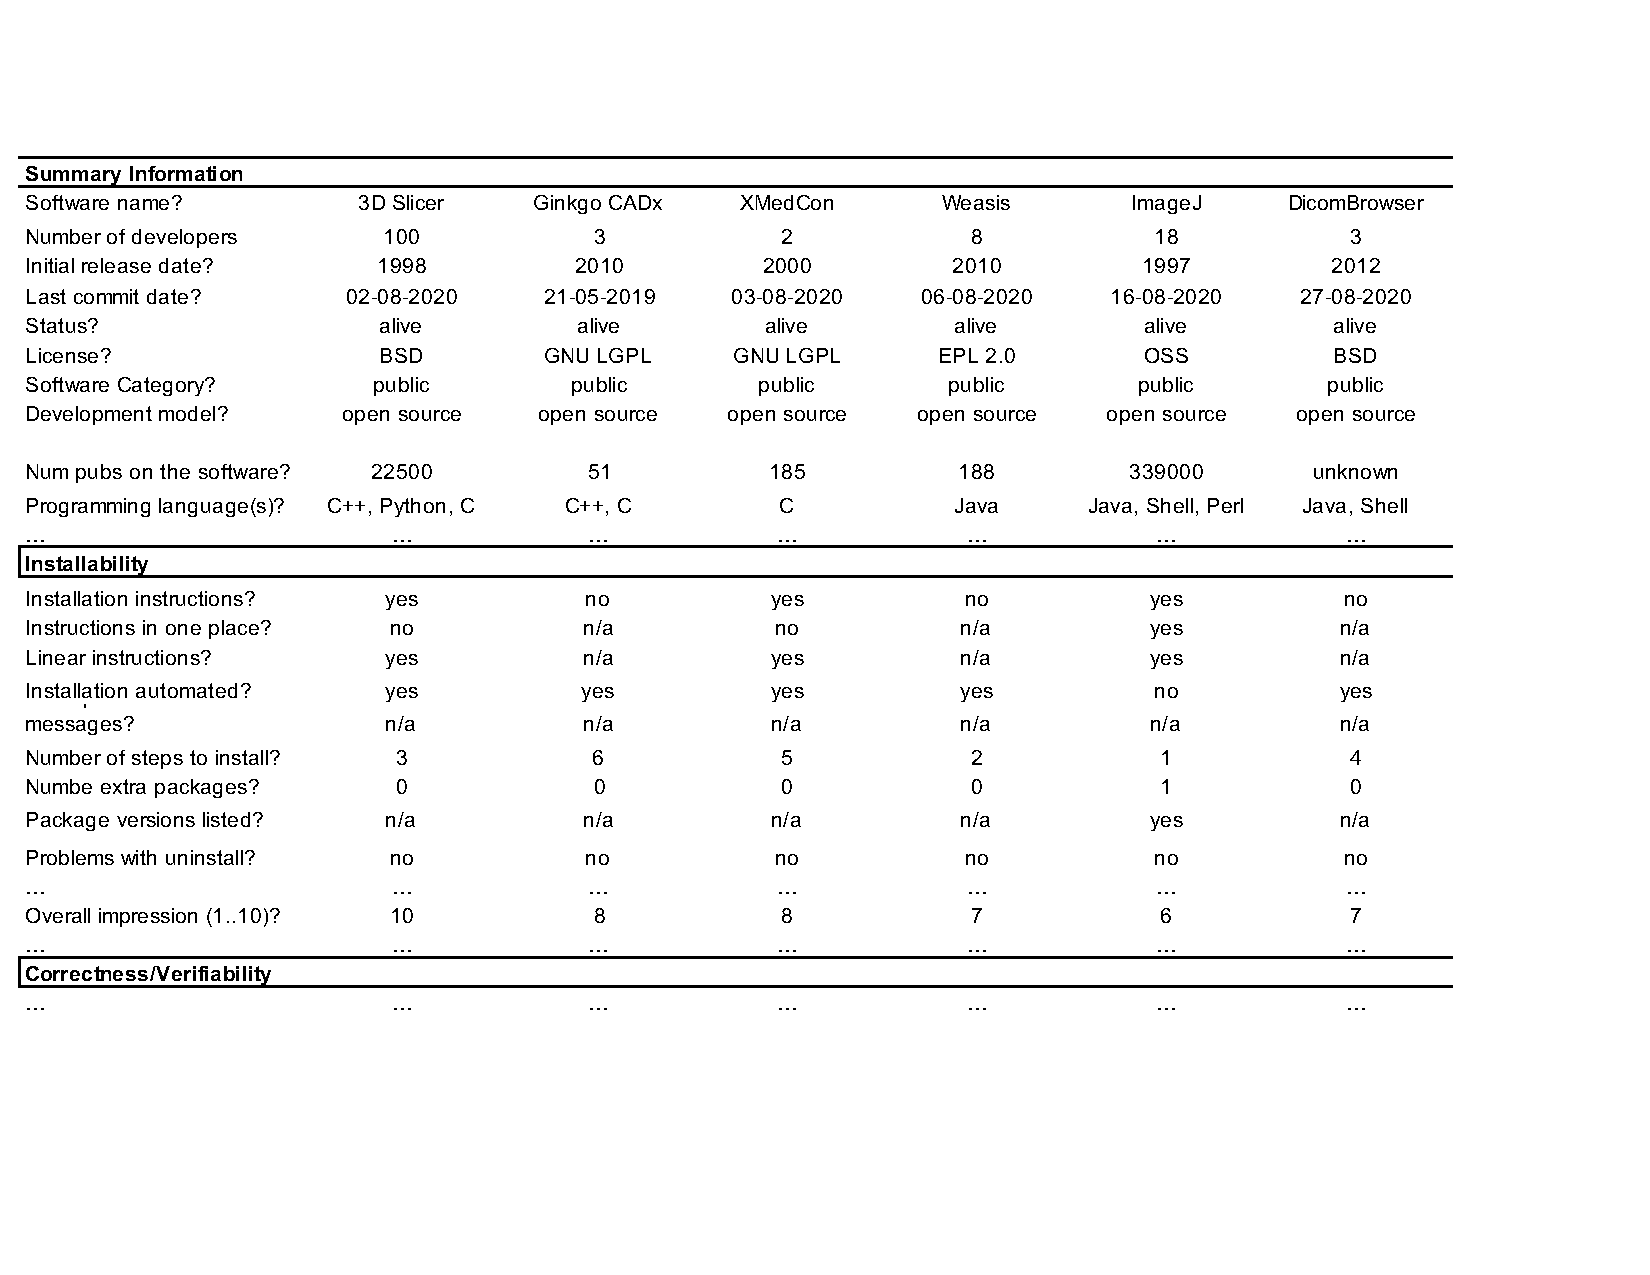
\includegraphics[scale=0.67]{figures/template.pdf}
\caption{Grading template example}
\label{fg_grading_template_example}
\end{figure}

The full template consists of 108 questions categorized under 9 qualities.  The
questions were designed to be unambiguous, quantifiable and measurable with
limited time and domain knowledge. The measures are grouped under headings for
each quality, and one for summary information. The summary information (shown in
Figure~\ref{fg_grading_template_example}) is the first section of the template.
This section summarizes general information, such as the software name, purpose,
platform, programming language, publications about the software, the first
release and the most recent change date, website, source code repository of the
product, number of developers, etc.  We follow the definitions given by
\citet{GewaltigAndCannon2012} for the software categories.  Public means
software intended for public use.  Private means software aimed only at a
specific group, while the concept category is used for software written simply
to demonstrate algorithms or concepts. The three categories of development
models are (open source, free-ware and commercial) are discussed in
Section~\ref{sec_software_categories}.  Information in the summary section sets
the context for the project, but it does not directly affect the grading scores.

For measuring each quality, we ask several questions and the typical answers are
among the collection of ``yes'', ``no'', ``n/a'', ``unclear'', a number, a
string, a date, a set of strings, etc. Each quality is assigned an overall
score, between 1 and 10, based on all the previous questions.  Several of the
qualities use the word ``surface''.  This is to highlight that, for these
qualities in particular, the best that we can do is a shallow measure.  For
instance, we are not currently doing any experiments to measure usability.
Instead, we are looking for an indication that usability was considered by the
developers.  We do this by looking for cues in the documentation, like a getting
started manual, a user manual and documentation of expected user
characteristics.  Below is a summary of how we assess adoption of best practices
by measuring each quality.

\begin{itemize}

\item \textbf{Installability} We assess the following: 
\begin{inparaenum}[i)]
    \item existence and quality of installation instructions;
    \item the quality of the user experience via the ease of following
    instructions, number of steps, automation tools; and,
    \item whether there is a means to verify the installation.
\end{inparaenum}
If any problem interrupts the process of installation or uninstallation, we give
a lower score. We also record the Operating System (OS) used for the
installation test.

\item \textbf{Correctness \& Verifiability} We check each project to identify
any techniques used to ensure this quality, such as literate programming,
automated testing, symbolic execution, model checking, unit tests, etc. We also
examine whether the projects use Continuous Integration and Continuous Delivery
(CI/CD). For verifiability, we go through the documents of the projects to check
for the presence of requirements specifications, theory manuals, and getting
started tutorials. If a getting started tutorial exists and provides expected
results, we follow it to check the correctness of the output.

\item \textbf{Surface Reliability} We check the following: 
\begin{inparaenum}[i)]
    \item whether the software breaks during installation;
    \item the operation of the software following the getting started tutorial
    (if present);
    \item whether the error messages are descriptive; and,
    \item whether we can recover the process after an error.
\end{inparaenum}

\item \textbf{Surface Robustness} We check how the software handles
unexpected/unanticipated input. For example, we prepare broken image files for
MI software packages that load image files. We use a text file (.txt) with a
modified extension name (.dcm) as an unexpected/unanticipated input. We load a
few correct input files to ensure the function is working correctly before
testing the unexpected/unanticipated ones.

\item \textbf{Surface Usability} We examine the project's documentation,
checking for the presence of getting started tutorials and/or a user manual. We
also check whether users have channels to request support, such as an e-mail
address, or issue tracker. Our impressions of usability are based on our
interaction with the software during testing.  In general, an easy-to-use
graphical user interface will score high.

\item \textbf{Maintainability} We believe that the artifacts of a project,
including source code, documents, and building scripts, significantly influence
its maintainability. Thus we check each project for the presence of such
artifacts as API documentation, bug tracker information, release notes, test
cases, and build scripts. We also check for the use of tools supporting issue
tracking and version control, the percentages of closed issues, and the
proportion of comment lines in the code.

\item \textbf{Reusability} We count the total number of code files for each
project. Projects with a large number of components potentially provide more
choices for reuse. Furthermore, well-modularized code, which tends to have
smaller parts in separate files, is typically easier to reuse. Thus, we assume
that projects with more code files and less Lines of Code (LOC) per file are
more reusable. We also consider projects with API documentation as delivering
better reusability.

\item \textbf{Surface Understandability} Given that time is a constraint, we
cannot look at all code files for each project; therefore, we randomly examine
10 code files for their understandability. We check the code's style within each
file, such as whether the identifiers, parameters, indentation, and formatting
are consistent, whether the constants (other than 0 and 1) are hardcoded, and
whether the code is modularized. We also check the descriptive information for
the code, such as documents mentioning the coding standard, the comments in the
code, and the descriptions or links for details on algorithms in the code. 

\item \textbf{Visibility/Transparency} To measure this quality, we check the
existing documents to find whether the software development process and
current status of a project are visible and transparent. We examine the
development process, current status, development environment, and release notes
for each project.
\end{itemize}

As part of filling in the measurement template, we use freeware tools to collect
repository related data. \href{https://github.com/tomgi/git_stats}{GitStats}
\citep{Gieniusz2019} is used to measure the number of binary files as well as
the number of added and deleted lines in a repository. This tool is also used to
measure the number of commits over different intervals of time.
\href{https://github.com/boyter/scc}{Sloc Cloc and Code (scc)}
\citep{Boyter2021} is used to measure the number of text based files as well as
the number of total, code, comment, and blank lines in a repository.

Both tools measure the number of text-based files in a git repository and lines
of text in these files. Based on our experience, most text-based files in a
repository contain programming source code, and developers use them to compile
and build software products. A minority of these files are instructions and
other documents. So we roughly regard the lines of text in text-based files as
lines of programming code. The two tools usually generate similar but not
identical results. From our understanding, this minor difference is due to the
different techniques to detect if a file is text-based or binary.

For projects on GitHub we manually collect additional information, such as the
numbers of stars, forks, people watching this repository, open pull requests,
closed pull requests, and the number of months a repository has been on GitHub.
We need to take care with the project creation date, since a repository can have
a creation date much earlier than the first day on GitHub.  For example, the
developers created the git repository for \textit{3D Slicer} in 2002, but did
not upload a copy of it to GitHub until 2020. Some GitHub data can be found
using its the GitHub Application Program Interface (API) via the following url:
\textit{https://api.github.com/repos/[owner]/[repository]} where [owner] and
[repository] are replaced by the repo specific values. The number of months a
repository has been on GitHub helps us understand the average change of metrics
over time, like the average new stars per month. 

The repository measures help us in many ways. Firstly, they help us get a fast
and accurate project overview. For example, the number of commits over the last
12 months shows how active a project has been, and the number of stars and forks
may reveal its popularity (used to assess \rqref{RQ_CompareHQ2Popular}).
Secondly, the results may affect our decisions regarding the grading scores for
some software qualities. For example, if the percentage of comment lines is low,
we double-check the understandability of the code; if the ratio of open versus
closed pull requests is high, we pay more attention to maintainability.

As in \citet{SmithEtAl2016}, Virtual machines (VMs) were used to provide an
optimal testing environments for each package. VMs were used because it is
easier to start with a fresh environment without having to worry about existing
libraries and conflicts. Moreover, when the tests are complete the VM can be
deleted, without any impact on the host operating system. The most significant
advantage of using VMs is to level the playing field. Every software install
starts from a clean slate, which removes ``works-on-my-computer'' errors. When
filling in the measurement template spreadsheet, the details for each VM
are noted, including hypervisor and operating system version.

When grading the software, we found 27 out of the 29 packages are compatible
with two or three different OSes, such as Windows, macOS, and Linux, and 5 of
them are browser-based, making them platform-independent. However, in the
interest of time, we only performed the measurements for each project by
installing it on one of the platforms.  When it was an option, we selected
Windows as the host OS.

\subsection{Interview Methods} \label{sec_interview_methods}

The measurement results summarize to this point are based on information we
collect from on-line resources. This information is incomplete because it
doesn't generally capture the development process, the developer pain points,
the perceived threats to software quality, and the developers' strategies to
address these threats.  Therefore, part of our methodology is to interview
developers.

Our interviews were guided by a list of 20 questions, which can be found in
\citet{SmithEtAl2021}. Some questions are about the background of the software,
the development teams, the interviewees, and how they organize the projects. We
also ask about the developer's understandings of the users. Some questions focus
on the current and past difficulties, and the solutions the team has found, or
will try. We also discuss the importance and current situations of
documentation. A few questions are about specific software qualities, such as
maintainability, understandability, usability, and reproducibility. The
interviews are semi-structured based on the question list; we ask follow-up
questions when necessary.  The interview process presented here was approved by
the McMaster University Research Ethics Board under the application number 
\href{https://github.com/smiths/AIMSS/blob/master/StateOfPractice/MACREM/Application.pdf}
{MREB\#: 5219}.

We sent interview requests to all 29 projects using contact information from
projects websites, code repository, publications, and from biographic pages at
the teams's institutions.  In the end nine developers from eight of the projects
agreed to participate: \textit{3D Slicer}, \textit{INVESALIUS 3}, \textit{dwv},
\textit{BioImage Suite Web}, \textit{ITK-SNAP}, \textit{MRIcroGL},
\textit{Weasis}, and \textit{OHIF}. We spent about 90 minutes for each
interview. One participant was too busy to have an interview, so they wrote down
their answers. In one case two developers from the same project agreed to be
interviewed. Meetings were held on-line using either Zoom or Teams, which
facilitated recording and automatic transcription of the meetings. The full
interview answers can be found in \citet{Dong2021}.

\section{Measurement Results} \label{ch_results}

Table \ref{tab_final_list} shows the 29 software packages that we measured,
along with summary data collected in the year 2020. We arrange the items in
descending order of LOC. We found the initial release dates (Rlsd) for most
projects and marked the two unknown dates with ``?''. We used the date of the
latest change to each code repository to decide the latest update. We found
funding information (Fnd) for only eight projects.  For the number of
contributors (NOC) we considered anyone who made at least one accepted commit as
a contributor. The NOC is not usually the same as the number of long-term
project members, since many projects received change requests and code from the
community.  With respect to the OS, 25 packages work on all three OSs: Windows
(W), macOS (M), and Linux (L). Although the usual approach to cross-platform
compatibility was to work natively on multiple OSes, five projects achieved
platform-independence via web applications. The full measurement data for all
packages is available in \citet{Dong2021-Data}.

\begin{table}[!ht]
\centering
\begin{tabular}{p{6cm}lllllllll}
\toprule
\multirow{2}{*}{Software} & \multirow{2}{*}{Rlsd} & \multirow{2}{*}{Updated} & \multirow{2}{*}{Fnd} & \multirow{2}{*}{NOC} & \multirow{2}{*}{LOC} & \multicolumn{3}{c}{OS} & \multirow{2}{*}{Web} \\ \cline{7-9}
 &  &  &  &  &  & W & M & L &  \\ \midrule
ParaView \citep{Ahrens2005} & 2002 & 2020-10 & X & 100 & 886326 & X & X & X & X \\
Gwyddion \citep{Nevcas2012} & 2004 & 2020-11 &  & 38 & 643427 & X & X & X &  \\
Horos \citep{horosproject2020} & ? & 2020-04 &  & 21 & 561617 &  & X &  &  \\
OsiriX Lite \citep{PixmeoSARL2019} & 2004 & 2019-11 &  & 9 & 544304 &  & X &  &  \\
3D Slicer \citep{Kikinis2014} & 1998 & 2020-08 & X & 100 & 501451 & X & X & X &  \\
Drishti \citep{Limaye2012} & 2012 & 2020-08 &  & 1 & 268168 & X & X & X &  \\
Ginkgo CADx \citep{Wollny2020} & 2010 & 2019-05 &  & 3 & 257144 & X & X & X &  \\
GATE \citep{Jan2004} & 2011 & 2020-10 &  & 45 & 207122 &  & X & X &  \\
3DimViewer \citep{TESCAN2020} & ? & 2020-03 & X & 3 & 178065 & X & X &  &  \\
medInria \citep{Fillard2012} & 2009 & 2020-11 &  & 21 & 148924 & X & X & X &  \\
BioImage Suite Web \citep{Papademetris2005} & 2018 & 2020-10 & X & 13 & 139699 &
X & X & X & X \\
Weasis \citep{Roduit2021} & 2010 & 2020-08 &  & 8 & 123272 & X & X & X &  \\
AMIDE \citep{Loening2017} & 2006 & 2017-01 &  & 4 & 102827 & X & X & X &  \\
XMedCon \citep{Nolf2003} & 2000 & 2020-08 &  & 2 & 96767 & X & X & X &  \\
ITK-SNAP \citep{Yushkevich2006} & 2006 & 2020-06 & X & 13 & 88530 & X & X & X &  \\
Papaya \citep{UTHSCSA2019} & 2012 & 2019-05 &  & 9 & 71831 & X & X & X &  \\
OHIF Viewer \citep{Ziegler2020} & 2015 & 2020-10 &  & 76 & 63951 & X & X & X & X \\
SMILI \citep{Chandra2018} & 2014 & 2020-06 &  & 9 & 62626 & X & X & X &  \\
INVESALIUS 3 \citep{Amorim2015} & 2009 & 2020-09 &  & 10 & 48605 & X & X & X &  \\
dwv \citep{Martelli2021} & 2012 & 2020-09 &  & 22 & 47815 & X & X & X & X \\
DICOM Viewer \citep{Afsar2021} & 2018 & 2020-04 & X & 5 & 30761 & X & X & X &  \\
MicroView \citep{ParallaxInnovations2020} & 2015 & 2020-08 &  & 2 & 27470 & X & X & X &  \\
MatrixUser \citep{Liu2016} & 2013 & 2018-07 &  & 1 & 23121 & X & X & X &  \\
Slice:Drop \citep{Haehn2013} & 2012 & 2020-04 &  & 3 & 19020 & X & X & X & X \\
dicompyler \citep{Panchal2010} & 2009 & 2020-01 &  & 2 & 15941 & X & X &  &  \\
Fiji \citep{Schindelin2012} & 2011 & 2020-08 & X & 55 & 10833 & X & X & X &  \\
ImageJ \citep{Rueden2017} & 1997 & 2020-08 & X & 18 & 9681 & X & X & X &  \\
MRIcroGL \citep{Rorden2021} & 2015 & 2020-08 &  & 2 & 8493 & X & X & X &  \\
DicomBrowser \citep{Archie2012} & 2012 & 2020-08 &  & 3 & 5505 & X & X & X &  \\ \bottomrule
\end{tabular}
\caption{Final software list (sorted in descending order of the number of Lines
Of Code (LOC))}
\label{tab_final_list}
\end{table}

Figure \ref{fig_language} shows the primary languages versus the number of
projects using them.  The primary language is the language used for the majority
of the project's code; in most cases projects also use other languages.  The
most popular language is C++, with almost 40\% of projects (11 of 29).  The two
least popular choices are Pascal and Matlab, with around 3\% of projects each
(1 of 29).

\begin{figure}[!ht]
\centering
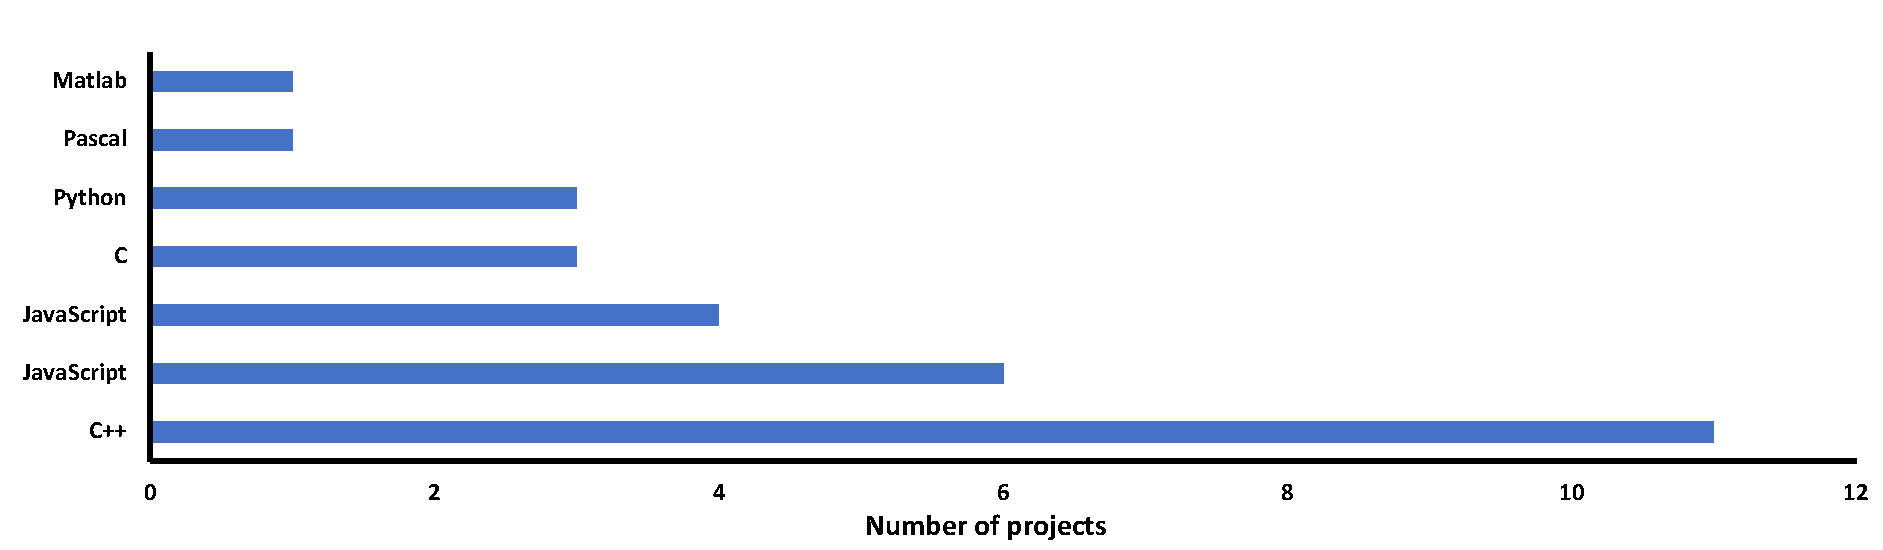
\includegraphics[scale=0.5]{figures/PrimaryLanguages.pdf}
\centering
\caption{\label{fig_language}Primary languages versus number of projects}
\end{figure}

\subsection{Installability} \label{sec_result_installability}

Figure \ref{fg_installability_scores} lists the installability scores.  We found
installation instructions for 16 projects. Among the ones without instructions,
\textit{BioImage Suite Web} and \textit{Slice:Drop} do not need installation,
since they are web applications. Installing 10 of the projects required extra
dependencies. Five of them are web applications (as shown in
Table~\ref{tab_final_list}) and depend on a browser; \textit{dwv}, \textit{OHIF
Viewer}, and \textit{GATE} needs extra dependencies to build; \textit{ImageJ}
and	\textit{Fiji} need an unzip tool; \textit{MatrixUser} is based on Matlab;
\textit{DICOM Viewer} needs to work on a Nextcloud platform.

\begin{figure}[!ht]
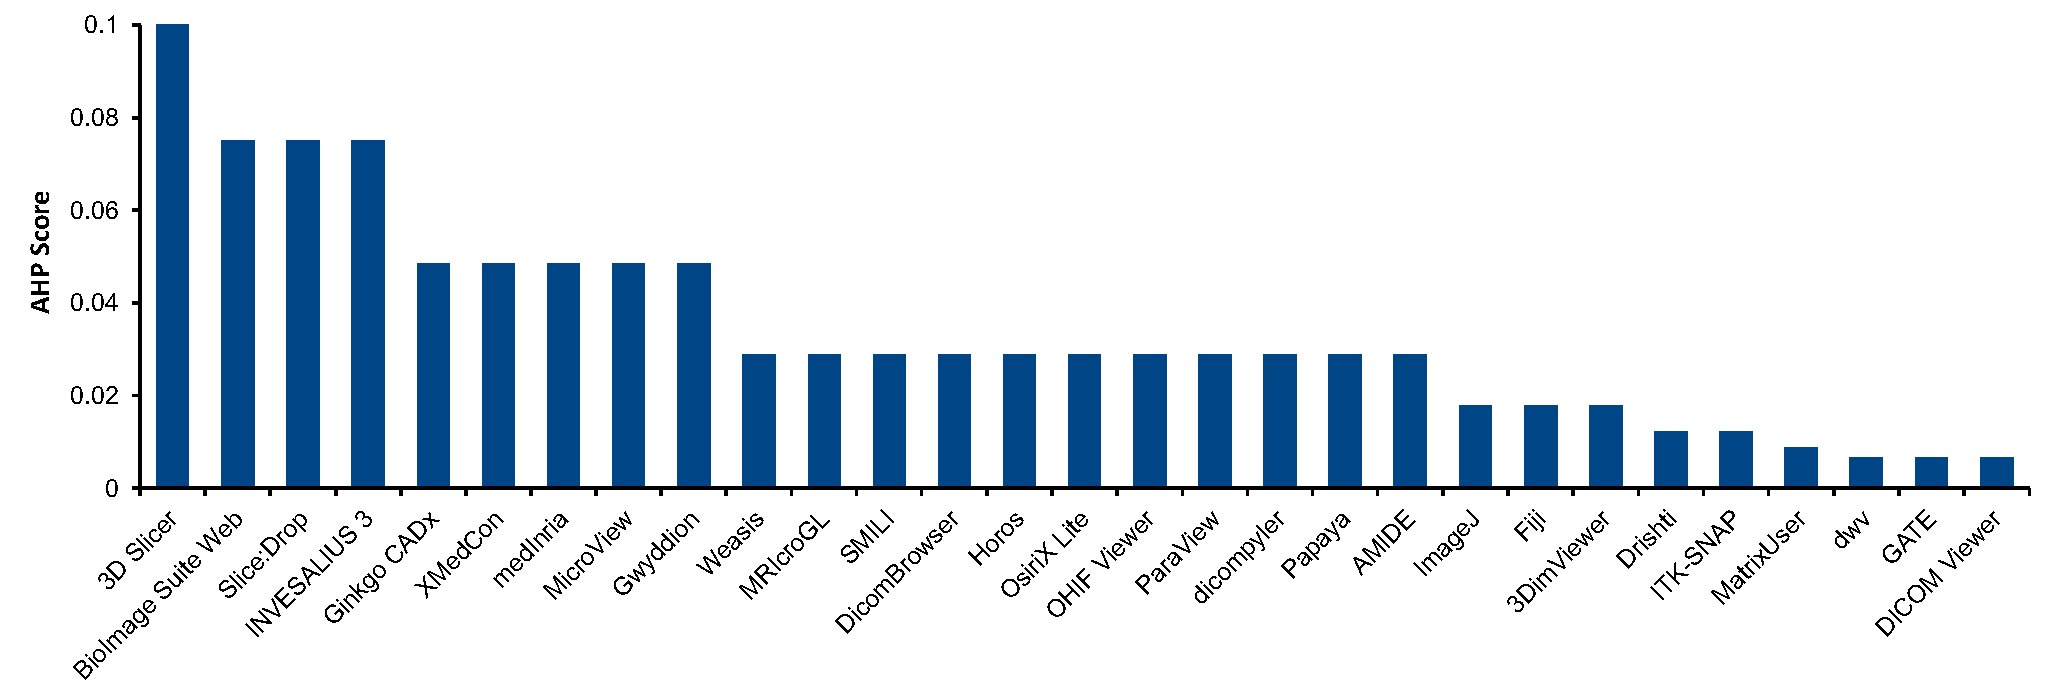
\includegraphics[scale=0.48]{figures/installability_scores.pdf}
\caption{AHP installability scores}
\label{fg_installability_scores}
\end{figure}

\textit{3D Slicer} has the highest score because it had easy to follow
installation instructions, and the installation processes were automated, fast,
and frustration-free, with all dependencies automatically added. There were also
no errors during the installation and uninstallation steps. Many other software
packages also had installation instructions and automated installers, and we had
no trouble installing them, such as \textit{INVESALIUS 3}, \textit{Gwyddion},
\textit{XMedCon}, and \textit{MicroView}. We determined their scores based on
the understandability of the instructions, installation steps, and user
experience. Since \textit{BioImage Suite Web} and \textit{Slice:Drop} needed no
installation, we gave them high scores. \textit{BioImage Suite Web} also
provided an option to download cache for offline usage, which was easy
to apply.

\textit{dwv}, \textit{GATE}, and \textit{DICOM Viewer} showed severe
installation problems. We were not able to install them, even after a reasonable
amount of time (2 hours).  For \textit{dwv} and \textit{GATE} we failed to build
from the source code, but we were able to proceed with measuring other qualities
using a deployed online version for \textit{dwv}, and a VM version for
\textit{GATE}. For \textit{DICOM Viewer} we could not install the NextCloud
dependency, and we did not have another option for running the software.
Therefore, for \textit{DICOM Viewer} we could not measure reliability or
robustness.  The other seven qualities could be measured, since they do not
require installation.

\textit{MatrixUser} has a lower score because it depended on Matlab. We assessed
the score from the point of view of a user that would have to install Matlab and
acquire a license.  Of course, for users that already work within Matlab, the
installability score should be higher.

\subsection{Correctness \& Verifiability} \label{sec_result_correctness_verifiability}

The scores of correctness \& verifiability are shown in
Figure~\ref{fg_correctness_verifiability_scores}. Generally speaking, the
packages with higher scores adopted more techniques to improve correctness, and
had better documentation for us to verify against.  For instance, we looked for
evidence of unit testing, since it benefits most parts of the software's life
cycle, such as designing, coding, debugging, and optimization
\citep{Hamill2004}.  We only found evidence of unit testing for about half of
the projects. We identified five projects using CI/CD tools: \textit{3D Slicer},
\textit{ImageJ}, \textit{Fiji}, \textit{dwv}, and \textit{OHIF Viewer}.

\begin{figure}[!ht]
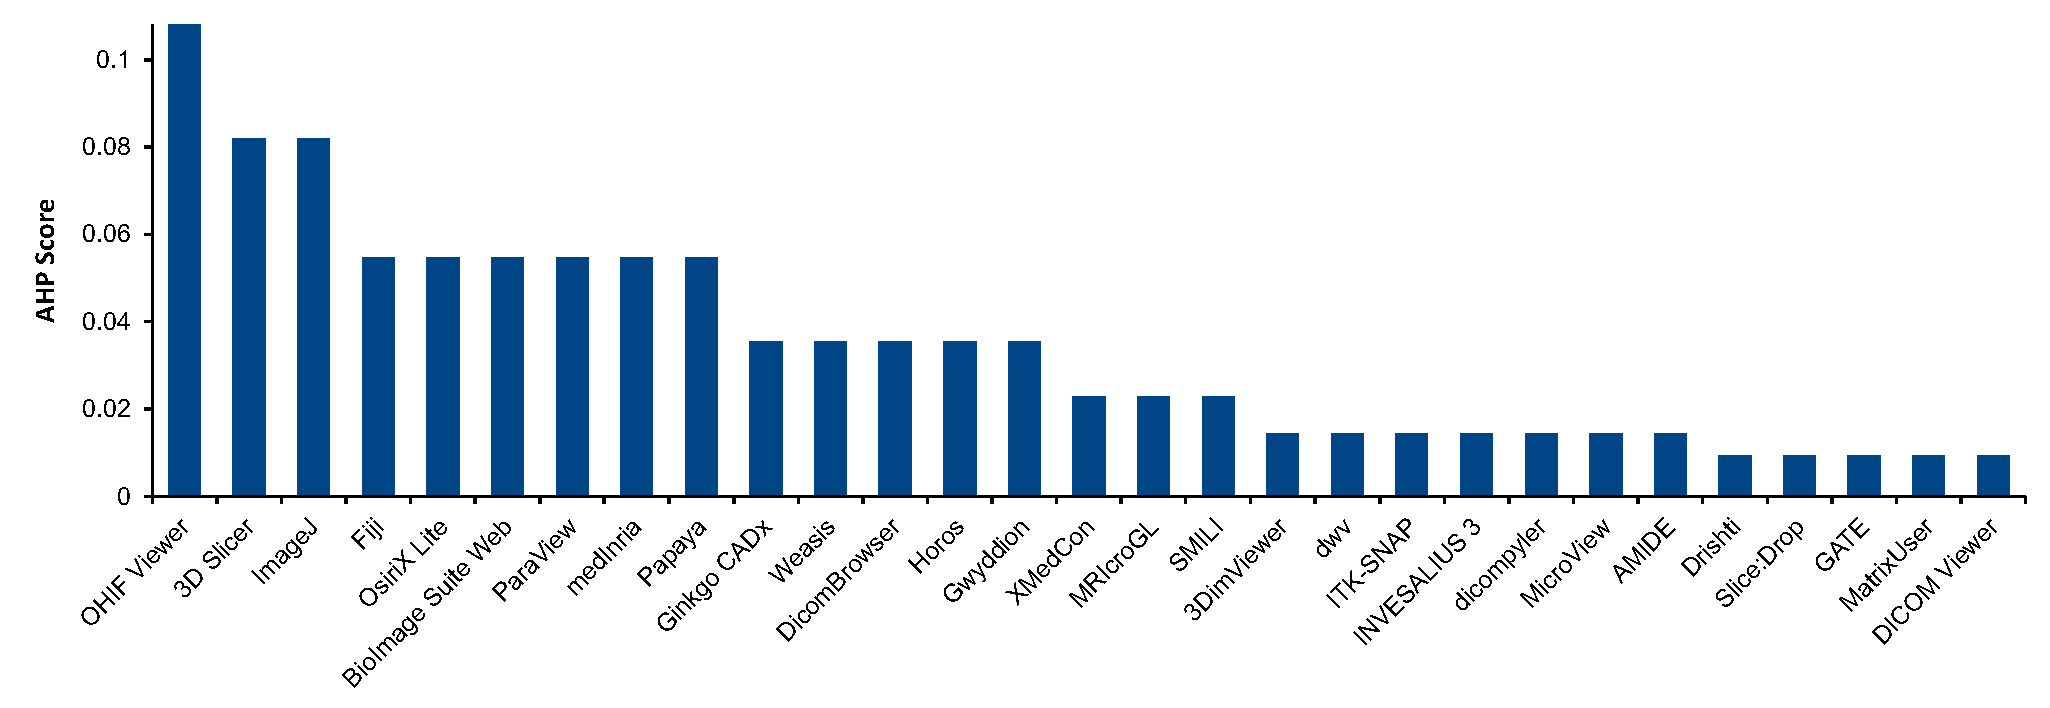
\includegraphics[scale=0.48]{figures/correctness_verifiability_scores.pdf}
\caption{AHP correctness \& verifiability scores}
\label{fg_correctness_verifiability_scores}
\end{figure}

Even for some projects with well-organized documents, requirements
specifications and theory manuals were still missing.  We could not identify
theory manuals for all projects and we did not find requirements specifications
for most projects. The only document we found was a road map of \textit{3D
Slicer}, which contained design requirements for upcoming changes.

\subsection{Surface Reliability} \label{sec_result_reliability}

Figure~\ref{fg_reliability_scores} shows the AHP results.  As shown in
Section~\ref{sec_result_installability}, most of the software products did not
``break'' during installation, or did not need installation; \textit{dwv} and
\textit{GATE} broke in the building stage, and the processes were not
recoverable; we could not install the dependency for \textit{DICOM Viewer}. Of
the seven software packages with a getting started tutorial and operation steps
in the tutorial, most showed no error when we followed the steps. However,
\textit{GATE} could not open macro files and became unresponsive several times,
without any descriptive error message. When assessing robustness
(Section~\ref{sec_result_robustness}), we found that \textit{Drishti} crashed
when loading damaged image files, without showing any descriptive error message.
On the other hand, we did not find any problems with the online version of
\textit{dwv}.

\begin{figure}[!ht]
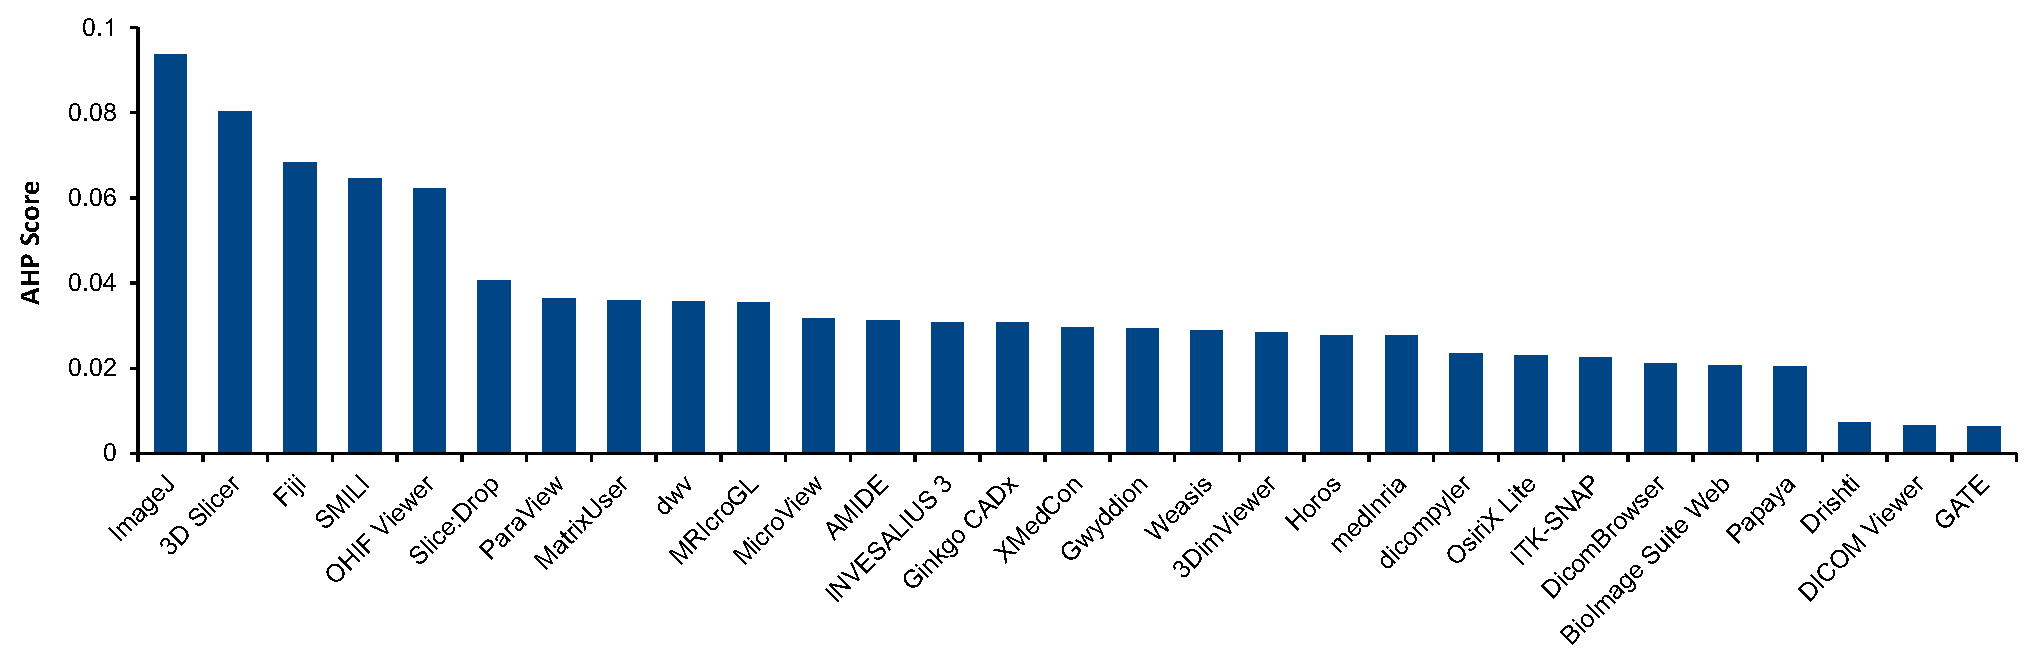
\includegraphics[scale=0.48]{figures/reliability_scores.pdf}
\caption{AHP surface reliability scores}
\label{fg_reliability_scores}
\end{figure}

\subsection{Surface Robustness} \label{sec_result_robustness}

Figure \ref{fg_robustness_scores} presents the scores for surface robustness.
The packages with higher scores elegantly handled unexpected/unanticipated
inputs, typically showing a clear error message. We may have underestimated the
score of \textit{OHIF Viewer}, since we needed further customization to load
data.

\begin{figure}[!ht]
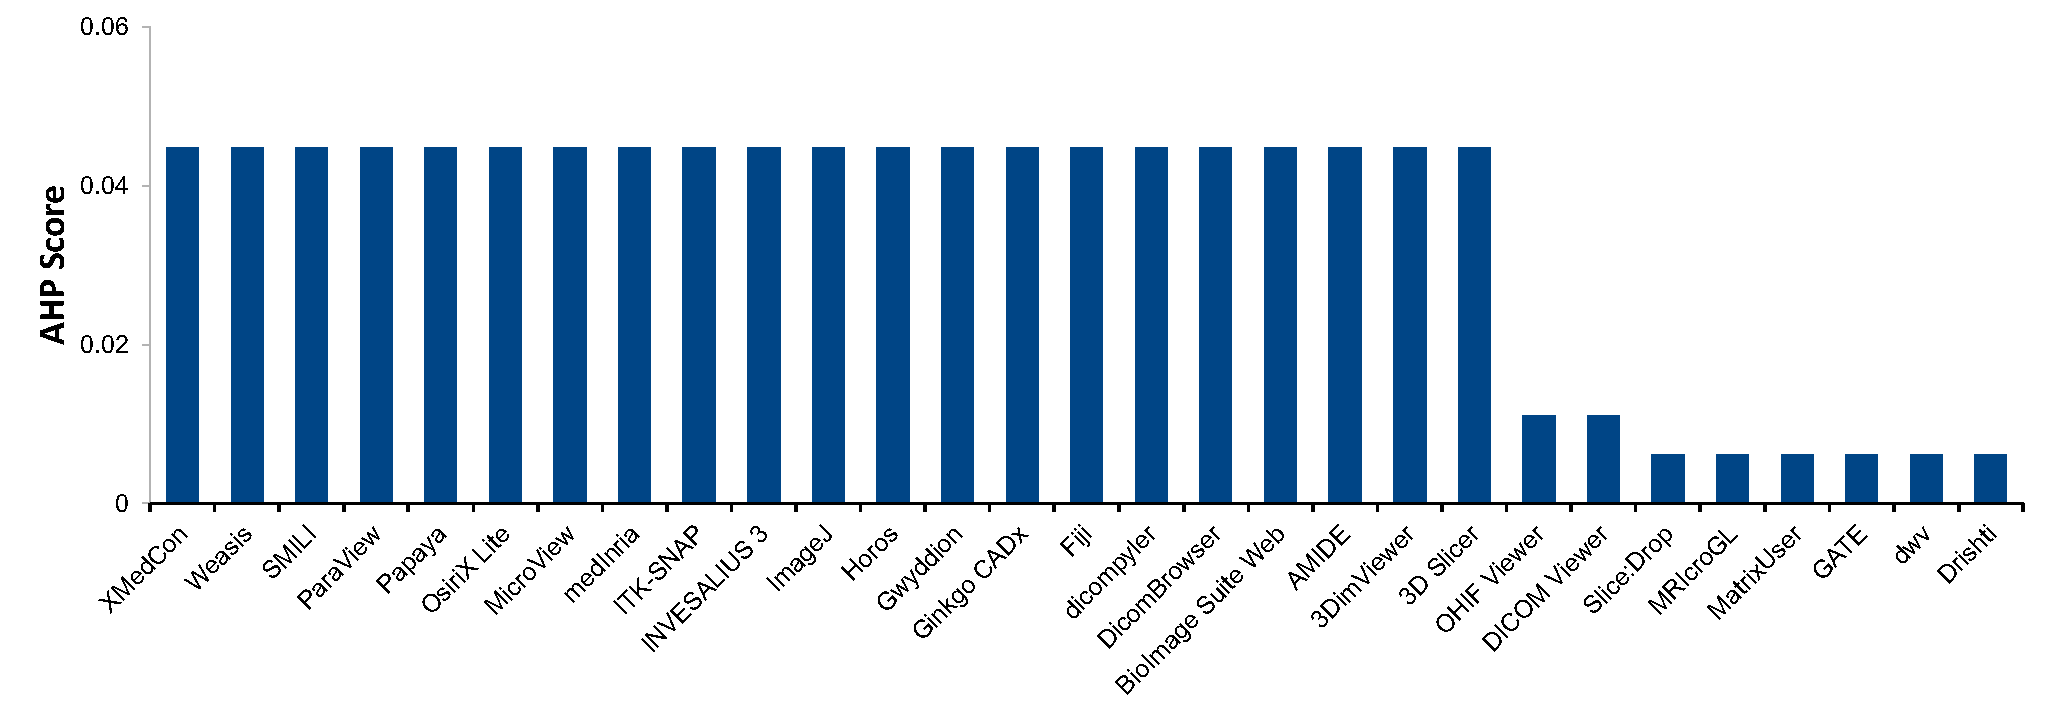
\includegraphics[scale=0.48]{figures/robustness_scores.pdf}
\caption{AHP surface robustness scores}
\label{fg_robustness_scores}
\end{figure}

Digital Imaging and Communications in Medicine (DICOM) ``defines the formats for
medical images that can be exchanged with the data and quality necessary for
clinical use'' \citep{MITA2021}. According to their documentation, all 29
software packages should support the DICOM standard. To test robustness, we
prepared two types of image files: correct and incorrect formats (with the
incorrect format created by relabelled a text file to have the ``.dcm''
extension).  All software packages loaded the correct format image, except for
\textit{GATE}, which failed for unknown reasons.  For the broken format,
\textit{MatrixUser}, \textit{dwv}, and \textit{Slice:Drop} ignored the incorrect
format of the file and loaded it regardless. They did not show any error message
and displayed a blank image. \textit{MRIcroGL} behaved similarly except that it
showed a meaningless image. \textit{Drishti} successfully detected the broken
format of the file, but the software crashed as a result.

\subsection{Surface Usability} \label{sec_result_usability}

Figure \ref{fg_usability_scores} shows the AHP scores for surface usability. The
software with higher scores usually provided both comprehensive documented
guidance and a good user experience. \textit{INVESALIUS 3} provided an excellent
example of a detailed and precise user manual. \textit{GATE} also provided a
large number of documents, but unfortunately we had difficulty understanding and
using them. We found getting started tutorials for only 11 projects, but a user
manual for 22 projects. \textit{MRIcroGL} was the only project that explicitly
documented expected user characteristics.

\begin{figure}[!ht]
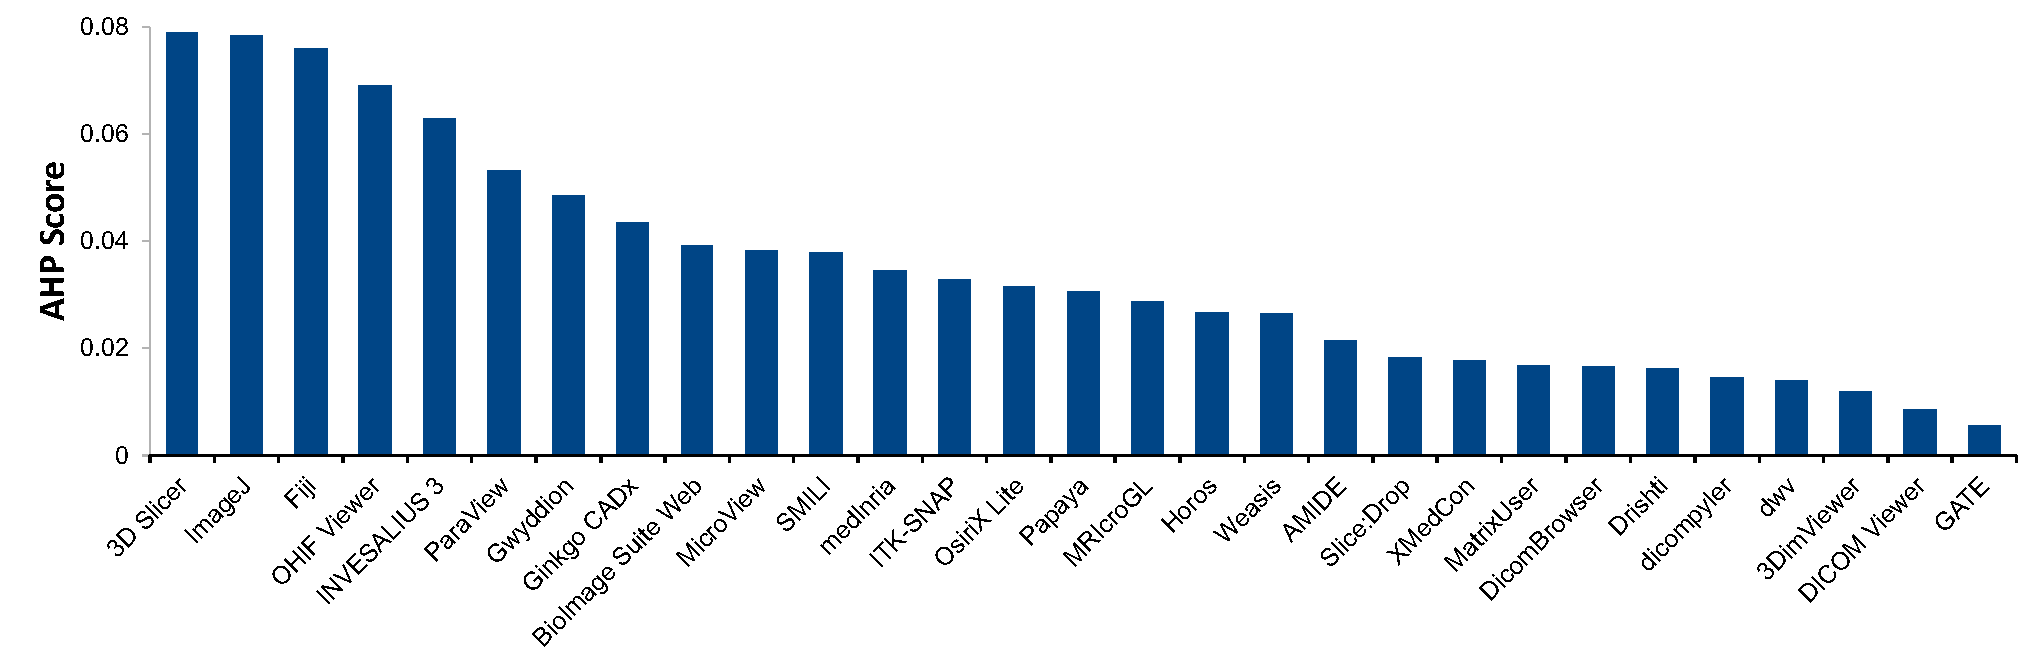
\includegraphics[scale=0.48]{figures/usability_scores.pdf}
\caption{AHP surface usability scores}
\label{fg_usability_scores}
\end{figure}
 
\subsection{Maintainability} \label{sec_score_maintainability}

Figure~\ref{fg_maintainability_scores} shows the ranking results for
maintainability. We marked \textit{3D Slicer} with the highest score because
we found it to have the most comprehensive artifacts. For example, as far as we
could find, only a few of the 29 projects had a product, developer's
manual, or API documentation, and only \textit{3D Slicer}, \textit{ImageJ},
\textit{Fiji} included all three documents. Moreover, \textit{3D Slicer} has a
much higher percentage of closed issues (91.65\%) compared to \textit{ImageJ}
(52.49\%) and \textit{Fiji} (63.79\%). Table~\ref{tab_maintainability_docs}
shows which projects had these documents, in the descending order of their
maintainability scores. 

\begin{figure}[!ht]
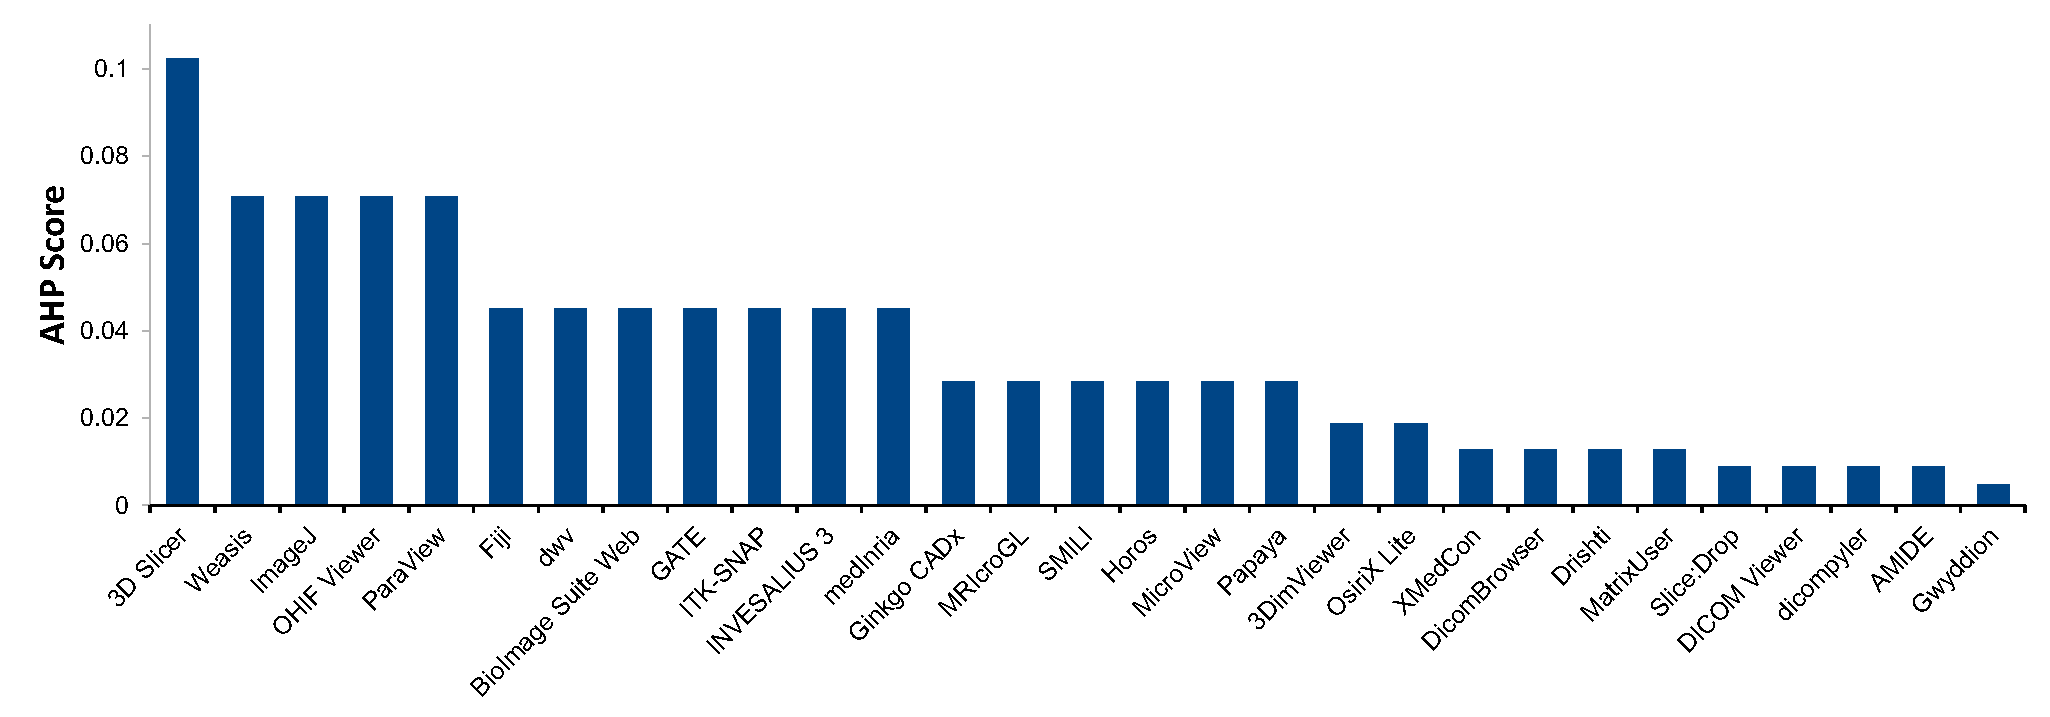
\includegraphics[scale=0.48]{figures/maintainability_scores.pdf}
\caption{AHP maintainability scores}
\label{fg_maintainability_scores}
\end{figure}

\begin{table}[!ht]
\centering
\begin{tabular}{lccc}
\toprule
\multicolumn{1}{c}{Software} & Prod.\ roadmap & Dev.\ manual & API doc. \\ 
\midrule
3D Slicer & X & X & X \\
ImageJ & X & X & X \\
Weasis &  & X &  \\
OHIF Viewer &  & X & X \\
Fiji & X & X & X \\
ParaView & X &  &  \\
SMILI &  &  & X \\
medInria &  & X &  \\
INVESALIUS 3 & X &  &  \\
dwv &  &  & X \\
BioImage Suite Web &  & X &  \\
Gwyddion &  & X & X \\ 
\bottomrule
\end{tabular}
\caption{Software with the maintainability documents (listed in descending order of 
maintainability score)}
\label{tab_maintainability_docs}
\end{table}

27 of the 29 projects used git as the version control tool, with 24 of these
using GitHub. \textit{AMIDE} used Mercurial and \textit{Gwyddion} used
Subversion. \textit{XMedCon}, \textit{AMIDE}, and \textit{Gwyddion} used
SourceForge. \textit{DicomBrowser} and \textit{3DimViewer} used BitBucket. 

\subsection{Reusability} \label{sec_result_reusability}

Figure~\ref{fg_reusability_scores} shows the AHP results for reusability. As
described in Section~\ref{sec_grading_software}, we gave higher scores to the
projects with API documentation. As shown in
Table~\ref{tab_maintainability_docs}, seven projects had API documents. We also
assumed that projects with more code files and less LOC per code file as more
reusable. Table \ref{tab_loc_per_file} shows the number of text-based files by
projects, which we used to approximate the number of code files. The table also
lists the total number of lines (including comments and blanks), LOC, and
average LOC per file. We arranged the items in descending order of their
reusability scores.

\begin{figure}[!ht]
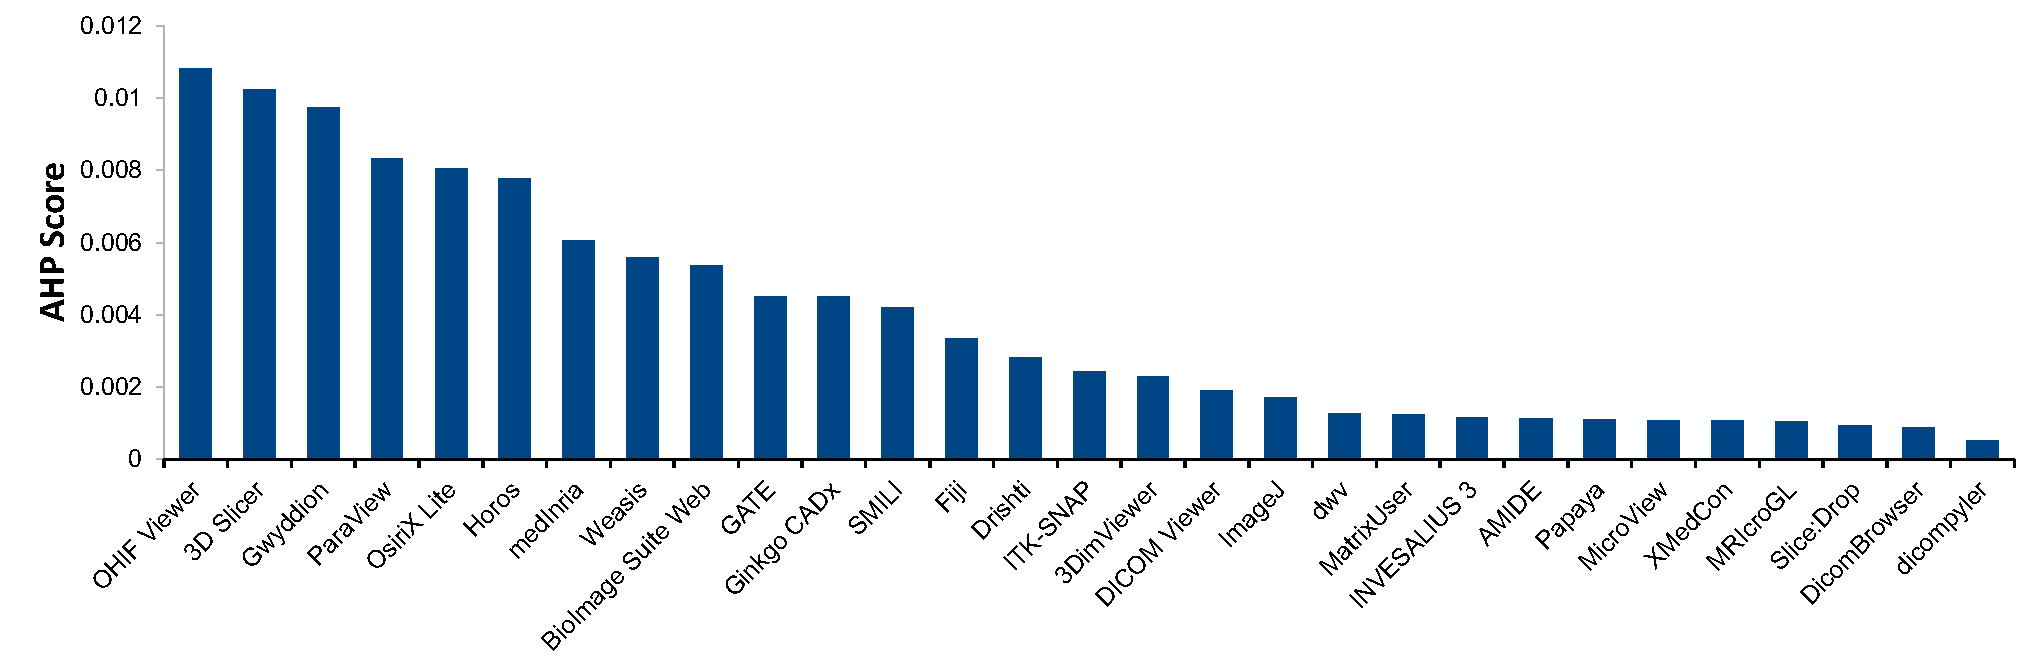
\includegraphics[scale=0.48]{figures/reusability_scores.pdf}
\caption{AHP reusability scores}
\label{fg_reusability_scores}
\end{figure}

\begin{table}[!ht]
\centering
\begin{tabular}{lllll}
\toprule
\multirow{2}{*}{Software} & \multirow{2}{*}{Text files} & \multirow{2}{*}{Total lines} & \multirow{2}{*}{LOC} & \multirow{2}{*}{LOC/file} \\
 &  &  &  &  \\ 
\midrule
OHIF Viewer & 1162 & 86306 & 63951 & 55 \\
3D Slicer & 3386 & 709143 & 501451 & 148 \\
Gwyddion & 2060 & 787966 & 643427 & 312 \\
ParaView & 5556 & 1276863 & 886326 & 160 \\
OsiriX Lite & 2270 & 873025 & 544304 & 240 \\
Horos & 2346 & 912496 & 561617 & 239 \\
medInria & 1678 & 214607 & 148924 & 89 \\
Weasis & 1027 & 156551 & 123272 & 120 \\
BioImage Suite Web & 931 & 203810 & 139699 & 150 \\
GATE & 1720 & 311703 & 207122 & 120 \\
Ginkgo CADx & 974 & 361207 & 257144 & 264 \\
SMILI & 275 & 90146 & 62626 & 228 \\
Fiji & 136 & 13764 & 10833 & 80 \\
Drishti & 757 & 345225 & 268168 & 354 \\
ITK-SNAP & 677 & 139880 & 88530 & 131 \\
3DimViewer & 730 & 240627 & 178065 & 244 \\
DICOM Viewer & 302 & 34701 & 30761 & 102 \\
ImageJ & 40 & 10740 & 9681 & 242 \\
dwv & 188 & 71099 & 47815 & 254 \\
MatrixUser & 216 & 31336 & 23121 & 107 \\
INVESALIUS 3 & 156 & 59328 & 48605 & 312 \\
AMIDE & 183 & 139658 & 102827 & 562 \\
Papaya & 110 & 95594 & 71831 & 653 \\
MicroView & 137 & 36173 & 27470 & 201 \\
XMedCon & 202 & 129991 & 96767 & 479 \\
MRIcroGL & 97 & 50445 & 8493 & 88 \\
Slice:Drop & 77 & 25720 & 19020 & 247 \\
DicomBrowser & 54 & 7375 & 5505 & 102 \\
dicompyler & 48 & 19201 & 15941 & 332 \\ 
\bottomrule
\end{tabular}
\caption{Number of files and lines (entries are sorted in descending order of
their reusability scores)}
\label{tab_loc_per_file}
\end{table}

\subsection{Surface Understandability} \label{sec_result_understandability}

Figure~\ref{fg_surface_understandability_scores} shows the scores for surface
understandability. All projects had a consistent coding style with parameters in
the same order for all functions; the code was modularized; the comments were
clear, indicating what is being done, not how. However, we only found explicit
identification of a coding standard for 3 out of the 29: \textit{3D Slicer},
\textit{Weasis}, and \textit{ImageJ}. We also found hard-coded constants (rather
than symbolic constants) in \textit{medInria}, \textit{dicompyler},
\textit{MicroView}, and \textit{Papaya}. We did not find any reference to the
algorithms used in projects \textit{XMedCon}, \textit{DicomBrowser},
\textit{3DimViewer}, \textit{BioImage Suite Web}, \textit{Slice:Drop},
\textit{MatrixUser}, \textit{DICOM Viewer}, \textit{dicompyler}, and
\textit{Papaya}. 

\begin{figure}[!ht]
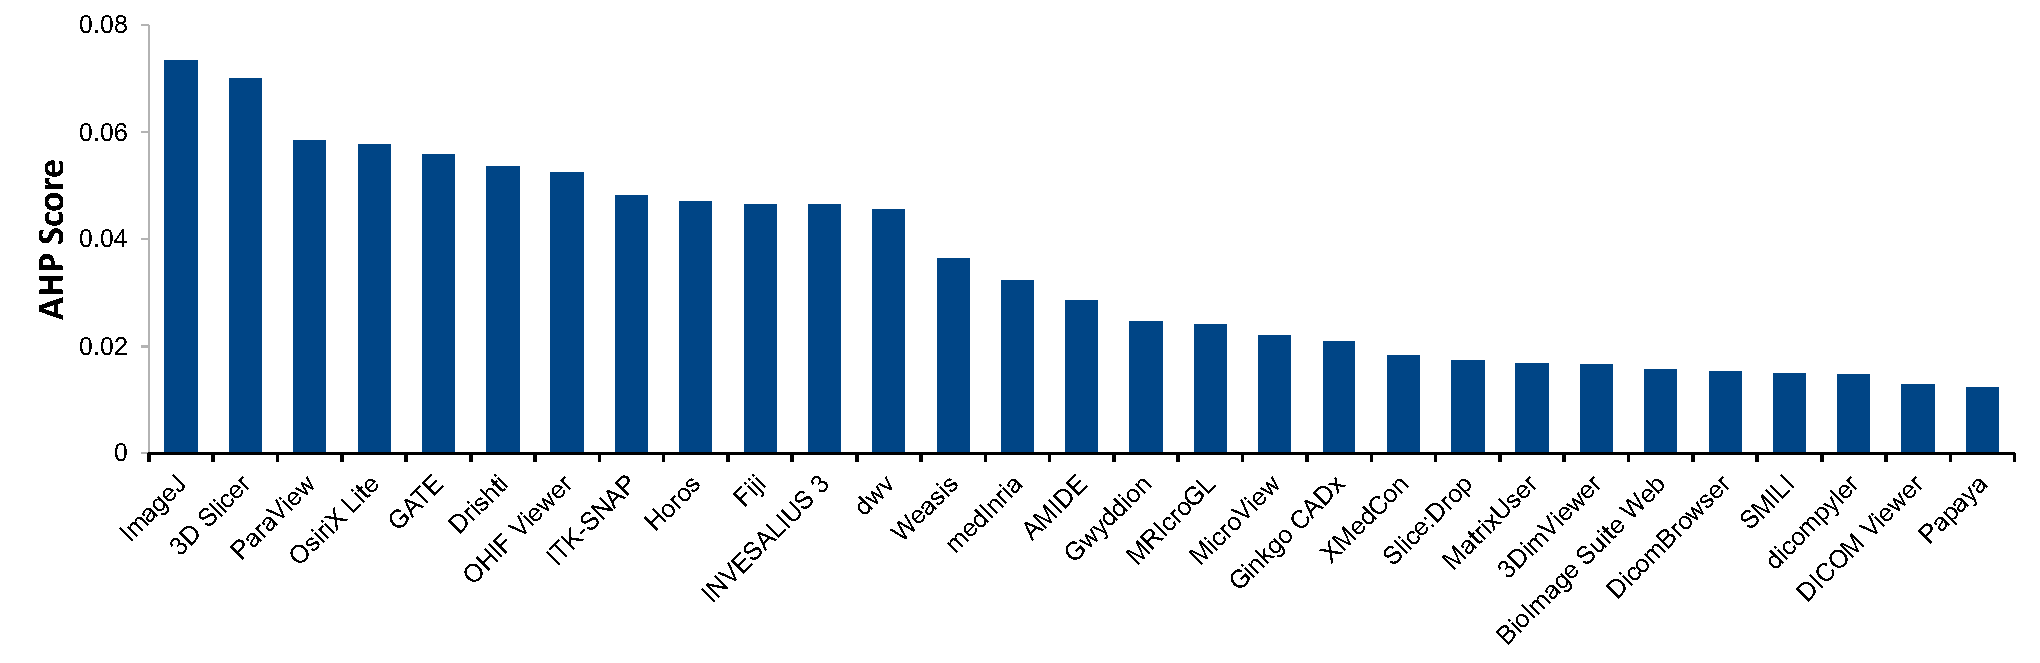
\includegraphics[scale=0.48]{figures/understandability_scores.pdf}
\caption{AHP surface understandability scores}
\label{fg_surface_understandability_scores}
\end{figure}

\subsection{Visibility/Transparency} \label{sec_result_visibility_transparency}

Figure~\ref{fg_visibility_transparency_scores} shows the AHP scores for
visibility/transparency. Generally speaking, the teams that actively documented
their development process and plans scored higher.
Table~\ref{tab_Visibility/Transparency_docs} shows the projects that had
documents for the development process, project status, development environment,
and release notes, in descending order of their visibility/transparency
scores.

\begin{figure}[!ht]
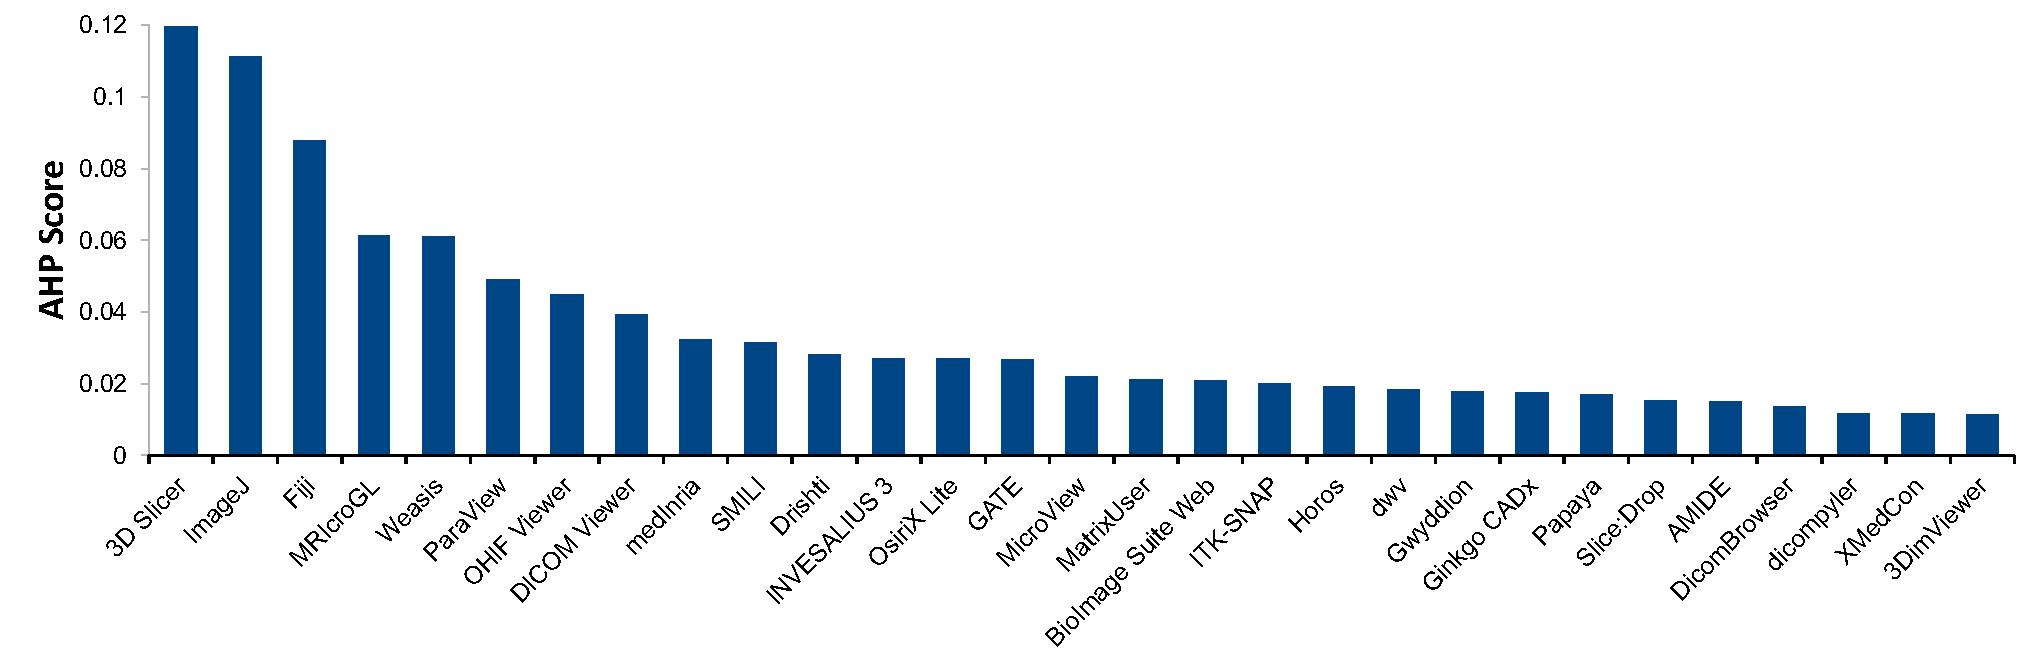
\includegraphics[scale=0.48]{figures/visibility_transparency_scores.pdf}
\caption{AHP visibility/transparency scores}
\label{fg_visibility_transparency_scores}
\end{figure}

\begin{table}[!ht]
\centering
\begin{tabular}{lllll}
\toprule
Software & Dev process & Proj status & Dev env & Rls notes \\ 
\midrule
3D Slicer & X & X & X & X \\
ImageJ & X & X & X & X \\
Fiji & X & X & X &  \\
MRIcroGL &  &  &  & X \\
Weasis &  &  & X & X \\
ParaView &  & X &  &  \\
OHIF Viewer &  &  & X & X \\
DICOM Viewer &  &  & X & X \\
medInria &  &  & X & X \\
SMILI &  &  &  & X \\
Drishti &  &  &  & X \\
INVESALIUS 3 &  &  &  & X \\
OsiriX Lite &  &  &  & X \\
GATE &  &  &  & X \\
MicroView &  &  &  & X \\
MatrixUser &  &  &  & X \\
BioImage Suite Web &  &  & X &  \\
ITK-SNAP &  &  &  & X \\
Horos &  &  &  & X \\
dwv &  &  &  & X \\
Gwyddion &  &  &  & X \\ 
\bottomrule
\end{tabular}
\caption{Software with visibility/transparency related documents (software is
listed in descending order of visibility/transparency score)}
\label{tab_Visibility/Transparency_docs}
\end{table}

\subsection{Overall Scores}

As described in Section~\ref{sec_AHP}, for our AHP measurements, we have nine
criteria (qualities) and 29 alternatives (software packages). In the absence of
a specific real world context, we assumed all nine qualities are equally
important. Figure~\ref{fg_overall_scores} shows the overall scores in descending
order. Since we produced the scores from the AHP process, the total sum of the
29 scores is precisely 1.

\begin{figure}[!ht]
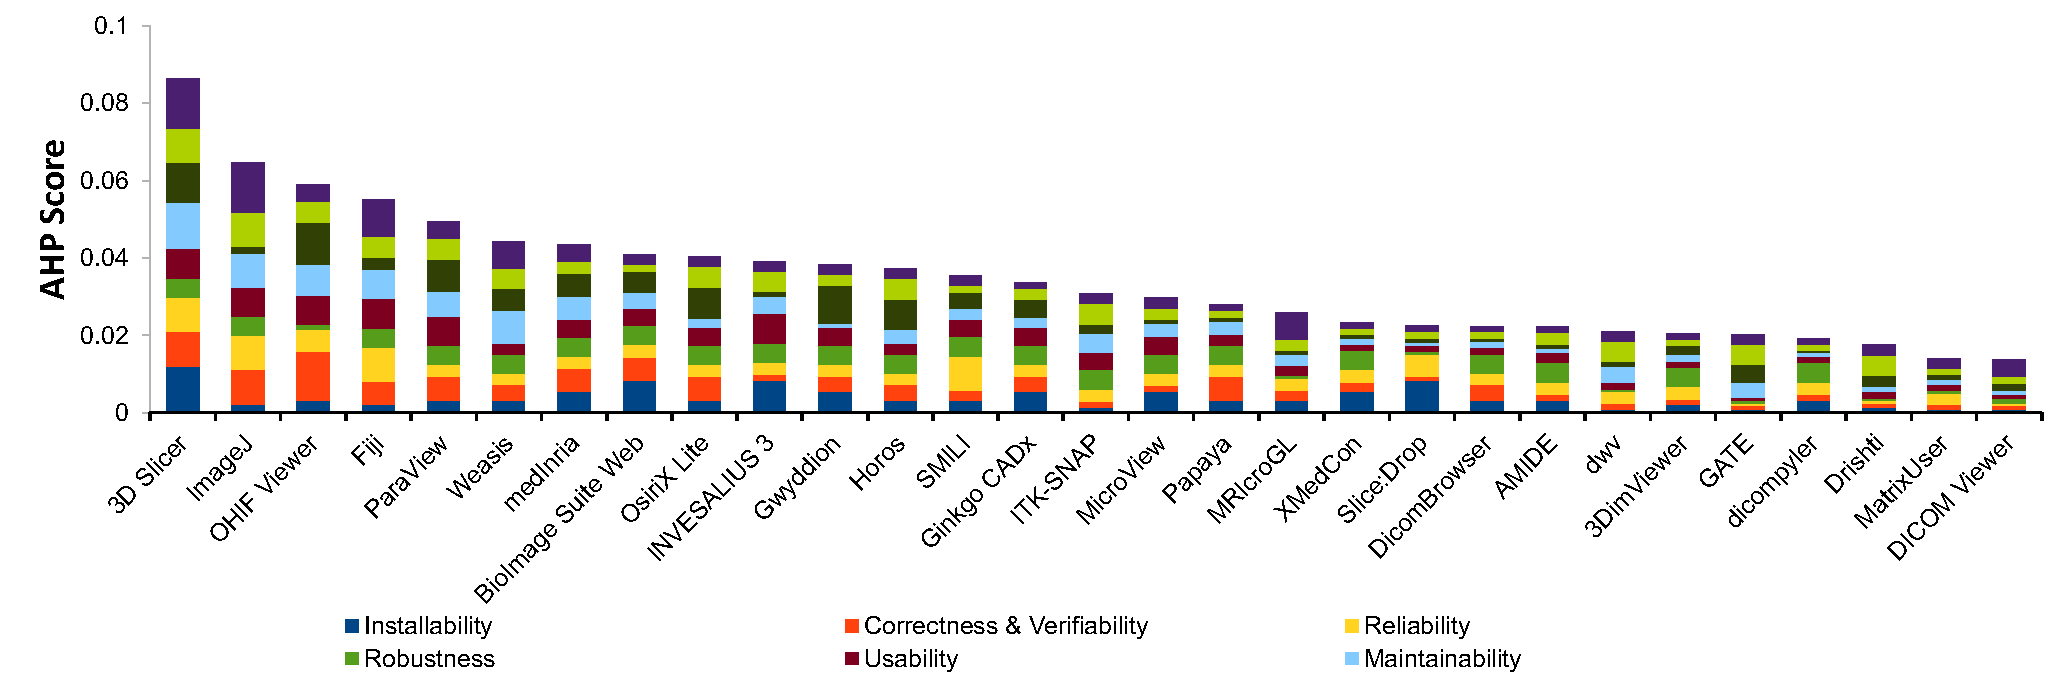
\includegraphics[scale=0.48]{figures/overall_scores.pdf}
\caption{Overall AHP scores with an equal weighting for all 9 software qualities}

\label{fg_overall_scores}
\end{figure}

The top three software products \textit{3D Slicer}, \textit{ImageJ}, and
\textit{OHIF Viewer} had higher scores in most criteria. \textit{3D Slicer}
ranked in the top two software products for all qualities except \textit{surface
robustness}; \textit{ImageJ} ranked in the top three for correctness \&
verifiability, surface reliability, surface usability, maintainability, surface
understandability, and visibility/transparency. \textit{OHIF Viewer} ranked in
the top five products for correctness \& verifiability, surface reliability,
surface usability, maintainability, and reusability. Given the installation
problems, we may have underestimated the scores on reliability and robustness
for \textit{DICOM Viewer}, but we compared it equally for the other seven
qualities.

\section{Comparison to Community Ranking} \label{Sec_VsCommunityRanking}

To address~\rqref{RQ_CompareHQ2Popular} about how our ranking compares to the
popularity of projects as judged by the scientific community, we make two
comparisons:
\begin{itemize}
\item A comparison of our ranking (from Section~\ref{ch_results}) with the
community ratings on GitHub, as shown by GitHub stars, number of forks, and
number of people watching the projects; and,
\item A comparison of top-rated software from our methodology with the top
recommendations from our domain experts (as mentioned in
Section~\ref{sec_software_selection}).
\end{itemize}

Table~\ref{tab_ranking_vs_GitHub} shows our ranking of the 29 MI projects, and
their GitHub metrics, if applicable. As mentioned in
Section~\ref{sec_score_maintainability}, 24 projects used GitHub. Since GitHub
repositories have different creation dates, we collect the number of months each
stayed on GitHub, and calculate the average number of new stars, people
watching, and forks per 12 months. The method of getting the creation date is
described in Section~\ref{sec_grading_software}.  The items in
Table~\ref{tab_ranking_vs_GitHub} are listed in descending order of the average
number of new stars per year.  The non-GitHub items are listed in the order of
our ranking.  All GitHub statistics were collected in July, 2021.  

Generally speaking, most of the top-ranking MI software projects also received
greater attention and popularity on GitHub. Between our ranking and the GitHub
stars-per-year ranking, four of the top five software projects appear in both
lists.Our top 5 packages are scattered among the first 8 positions on the GitHub
list. However, as discussed below there are discrepancies between the two lists.

In some cases projects are popular in the community, but were assigned a low
rank by our methodology.  This is the case for \textit{dwv}. The reason for the
low ranking is that, as mentioned in Section~\ref{sec_result_installability}, we
failed to build it locally, and used the test version on its websites for the
measurements. We followed the instructions and tried to run the command ``yarn
run test'' locally, which did not work. In addition, the test version did not
detect a broken DICOM file and displayed a blank image as described in
Section~\ref{sec_result_robustness}. We might underestimate the scores for
\textit{dwv} due to uncommon technical issues. We also ranked \textit{DICOM
Viewer} much lower than its popularity. As mentioned in
Section~\ref{sec_result_installability} it depended on the NextCloud platform
that we could not successfully install. Thus, we might underestimate the scores
of its surface reliability and surface robustness. In addition, we weighted all
qualities equally, which is not likely to be the case with all users. As a
result, some projects with high community popularity may have scored lower with
our method because of a relatively higher (compared to the scientific
community's implicit ranking) weighting of the poor scores for some qualities. A
further explanation for discrepancies between our measures and the star measures
may also be due to inaccuracy with using stars to approximate popularity.  Stars
are not an ideal measure because stars represent the community's feeling in the
past more than they measure current preferences \citep{Szulik2017}.  The issue
with stars is that they tend only to be added, not removed.  A final reason for
inconsistencies between our ranking and the community's ranking is that, as for
consumer products, more factors influence popularity than just quality.

\begingroup
\renewcommand{\arraystretch}{0.85}
\begin{table}[!ht]
\centering
\begin{tabular}{llllll}
\toprule
Software & Comm.\ rank & Our rank & Stars/yr & Watches/yr & Forks/yr \\ 
\midrule
3D Slicer & 1 & 1 & 284 & 19 & 128 \\
OHIF Viewer & 2 & 3 & 277 & 19 & 224 \\
dwv & 3 & 23 & 124 & 12 & 51 \\
ImageJ & 4 & 2 & 84 & 9 & 30 \\
ParaView & 5 & 5 & 67 & 7 & 28 \\
Horos & 6 & 12 & 49 & 9 & 18 \\
Papaya & 7 & 17 & 45 & 5 & 20 \\
Fiji & 8 & 4 & 44 & 5 & 21 \\
DICOM Viewer & 9 & 29 & 43 & 6 & 9 \\
INVESALIUS 3 & 10 & 10 & 40 & 4 & 17 \\
Weasis & 11 & 6 & 36 & 5 & 19 \\
dicompyler & 12 & 26 & 35 & 5 & 14 \\
OsiriX Lite & 13 & 9 & 34 & 9 & 24 \\
MRIcroGL & 14 & 18 & 24 & 3 & 3 \\
GATE & 15 & 25 & 19 & 6 & 26 \\
Ginkgo CADx & 16 & 14 & 19 & 4 & 6 \\
BioImage Suite Web & 17 & 8 & 18 & 5 & 7 \\
Drishti & 18 & 27 & 16 & 4 & 4 \\
Slice:Drop & 19 & 20 & 10 & 2 & 5 \\
ITK-SNAP & 20 & 15 & 9 & 1 & 4 \\
medInria & 21 & 7 & 7 & 3 & 6 \\
SMILI & 22 & 13 & 3 & 1 & 2 \\
MatrixUser & 23 & 28 & 2 & 0 & 0 \\
MicroView & 24 & 16 & 1 & 1 & 1 \\
Gwyddion & 25 & 11 & n/a & n/a & n/a \\
XMedCon & 26 & 19 & n/a & n/a & n/a \\
DicomBrowser & 27 & 21 & n/a & n/a & n/a \\
AMIDE & 28 & 22 & n/a & n/a & n/a \\
3DimViewer & 29 & 24 & n/a & n/a & n/a \\ 
\bottomrule
\end{tabular}
\caption{Software ranking by our methodology versus the community (Comm.)
ranking using GitHub metrics (Sorted in descending order of community
popularity, as estimated by the number of new stars per year)}
\label{tab_ranking_vs_GitHub}
\end{table}
\endgroup

As shown in Section~\ref{sec_software_selection}, our domain experts recommended
a list of top software with 12 software products.  All of the top 4 entries from
the Domain Expert's list are among the top 12 ranked by our methodology. Three
of the top four on both lists are the same: \textit{3D Slicer}, \textit{ImageJ},
and \textit{Fiji}. \textit{3D Slicer} is top project by both rankings (and by
the GithHub stars measure as well).  The Domain Expert ranked \textit{Horos} as
their second choice, while we ranked it twelfth.  Our third ranked project,
\textit{OHIF Viewer} was not listed by the Domain Expert.  Neither were the
software packages that we ranked from fifth to eleventh (\textit{ParaView},
\textit{Weasis}, \textit{medInria}, \textit{BioImage Suite Web}, \textit{OsiriX
Lite}, \textit{INVESALIUS}, and \textit{Gwyddion}).  The software mentioned by
the Domain Expert that we did not rank were the six recommended packages that
did not have visualization as the primary function (as discussed in
Section~\ref{sec_software_selection}).  The differences between the list
recommended by our methodology and the Domain Expert are not surprising.  As
mentioned above, the methodology weights all qualities equally, but that may not
be the case for the Domain Expert's impressions.  Moreover, although the Domain
Expert has significant experience with MI software, he has not used every one of
the 29 packages that were measured.

Although our ranking and the estimate of the community's ranking are not perfect
measures, they do suggest a correlation between best practices and popularity.
We do not know which comes first, the use of best practices or popularity, but
we do know that the top ranked packages tend to incorporate best practices. The
next sections will explore how the practices of the MI community compare to the
broader research software community. We will also investigate the practices from
the top projects that others within the MI community, and within the broader
research software community, can potentially adopt.

\section{Comparison Between MI and Research Software for Artifacts}
\label{Sec_CompareArtifacts}

As part of filling in the measurement template (from
Section~\ref{sec_grading_software}) we summarized the artifacts observed in each
MI package. Table~\ref{artifactspresent} groups the artifacts by frequency into
categories of common (20 to 29 ($>$67\%) packages), uncommon (10 to 19 (33-67\%)
packages), and rare (1 to 9 ($<$33\%) packages). The full measurements are
summarized in \citet{Dong2021-Data}.  The details on which projects use which
types of artifacts are summarized in Tables~\ref{tab_maintainability_docs}
and~\ref{tab_Visibility/Transparency_docs} for documents related to
maintainability and visibility, respectively.

\begin{table}[ht!]
    \begin{center}
    \begin{tabular}{ p{4.6 cm} p{5.6 cm} p{5 cm}}
    \toprule
    \textbf{Common} & \textbf{Uncommon} & \textbf{Rare} \\
    \midrule
    README (29) & Build scripts (18) & Getting Started (9)\\
    Version control (29) & Tutorials (18) & Developer's manual (8)\\
    License (28) & Installation guide (16) & Contributing (8)\\
    Issue tracker (28) & Test cases (15) & API documentation (7)\\
    User manual (22) & Authors (14) & Dependency list (7)\\
    Release info. (22) & Frequently Asked Questions (FAQ) (14) & Troubleshooting guide (6)\\
     & Acknowledgements (12) & Product roadmap (5)\\
     & Changelog (12) & Design documentation (5)\\
     & Citation (11) & Code style guide (3)\\
     & & Code of conduct (1)\\
     & & Requirements (1)\\
    \bottomrule
    \end{tabular}
    \caption{Artifacts Present in MI Packages, Classified by Frequency (The number 
    in brackets is the number of occurrences)}
    \label{artifactspresent}
    \end{center}
\end{table}

We answer~\rqref{RQ_CompareArtifacts} by comparing the artifacts that we
observed in MI repositories to those observed and recommended for research
software in general. Our comparison may point out areas where some MI software
packages fall short of current best practices. This is not intended to be a
criticism of any existing packages, especially since in practice not every
project needs to achieve the highest possible quality. However, rather than
delve into the nuances of which software can justify compromising which
practices we will write our comparison under the ideal assumption that every
project has sufficient resources to match best practices.
    
Table~\ref{Tbl_Guidelines} (based on data from \citep{SmithAndMichalski2022})
shows that MI artifacts generally match the recommendations found in nine
current research software development guidelines:
\begin{itemize}
\item United States Geological Survey Software Planning Checklist
\citep{USGS2019},
\item DLR (German Aerospace Centre) Software Engineering Guidelines
\citep{TobiasEtAl2018}, 
\item Scottish Covid-19 Response Consortium Software Checklist
\citep{BrettEtAl2021},
\item Good Enough Practices in Scientific Computing \citep{WilsonEtAl2016},
\item xSDK (Extreme-scale Scientific Software Development Kit) Community Package
Policies \citep{SmithAndRoscoe2018},
\item Trilinos Developers Guide \citep{HerouxEtAl2008},
\item EURISE (European Research Infrastructure Software Engineers') Network
Technical Reference \citep{ThielEtAl2020},
\item CLARIAH (Common Lab Research Infrastructure for the Arts and Humanities)
Guidelines for Software Quality \citep{vanGompelEtAl2016}, and
\item A Set of Common Software Quality Assurance Baseline Criteria for Research
Projects \citep{OrvizEtAl2017}.
\end{itemize}

In Table~\ref{Tbl_Guidelines} each row corresponds to an artifact.  For a given
row, a checkmark in one of the columns means that the corresponding guideline
recommends this artifact.  The last column shows whether the artifact appears in
the measured set of MI software, either not at all (blank), commonly (C),
uncommonly (U) or rarely (R).  We did our best to interpret the meaning of each
artifact consistently between guidelines and specific MI software, but the
terminology and the contents of artifacts are not standardized.  The challenge
even exists for the ubiquitous README file.  As illustrated by
\citet{PranaEtAl2018}, the content of README files shows significant variation
between projects.  Although some content is reasonably consistent, with 97\% of
README files contain at least one section describing the `What` of the
repository and 89\% offering some `How` content, other categories are more
variable.  For instance, information on `Contribution`, `Why`', and `Who`,
appear in 28\%, 26\% and 53\% of the analyzed files, respectively
\citep{PranaEtAl2018}.  

The frequency of checkmarks in Table~\ref{Tbl_Guidelines} indicates the
popularity of recommending a given artifact, but it does not imply that the most
commonly recommended artifacts are the most important artifacts. Just because an
artifact is not explicitly recommended in a given guidelines, does not mean that
the artifact is not valued by the guideline authors.  They may have excluded it
because it is out of the scope of their recommendations, or outside of their
experience.  For instance, an artifact related to uninstall is only explicitly
mentioned by \citep{vanGompelEtAl2016}), but other guideline authors would
likely see its value.  They may simply feel that uninstall is implied by
install, or they may have never asked themselves whether separate uninstall
instructions are needed.

\begin{table}[!ht]
\begin{center}
\begin{tabular}{ p{2.5cm}p{1cm}p{1cm}p{1cm}p{1cm}p{1cm}p{1cm}p{1cm}p{1.2cm}p{1cm}p{0.8cm} }
\toprule
~ \ & \cite{USGS2019} & \cite{TobiasEtAl2018} & \cite{BrettEtAl2021} &
\cite{WilsonEtAl2016} & \cite{SmithAndRoscoe2018} & \cite{HerouxEtAl2008} &
\cite{ThielEtAl2020} & \cite{vanGompelEtAl2016} & \cite{OrvizEtAl2017} & MI\\
\midrule
LICENSE & \checkmark & \checkmark & \checkmark & \checkmark & \checkmark & &
\checkmark & \checkmark & \checkmark & C\\
README &  & \checkmark & \checkmark & \checkmark & \checkmark & & \checkmark &
\checkmark & \checkmark & C\\
CONTRIBUTING &  & \checkmark & \checkmark & \checkmark & \checkmark & &
\checkmark & \checkmark & \checkmark & R\\
CITATION &  &  &  & \checkmark & & & & \checkmark & \checkmark & U\\
CHANGELOG &  & \checkmark &  & \checkmark & \checkmark & & \checkmark &  &  & U\\
INSTALL &  &  &  &  & \checkmark & & \checkmark & \checkmark & \checkmark & U\\
\midrule
Uninstall &  &  &  &  & & & & \checkmark & &  \\
Dependency List &  &  & \checkmark & & \checkmark & & & \checkmark &  & R\\
Authors &  &  &  &  &  &  & \checkmark & \checkmark & \checkmark & U\\
Code of Conduct &  &  &  &  & & & \checkmark & & & R\\
Acknowledgements &  &  &  &  &  &  & \checkmark & \checkmark & \checkmark & U\\
Code Style Guide &  & \checkmark &  &  & & & \checkmark & \checkmark & \checkmark & R\\
Release Info. &  & \checkmark &  &  & & \checkmark & \checkmark & & & C\\
Prod.\ Roadmap &  &  &  &  & & \checkmark & \checkmark & \checkmark & & R\\
\midrule
Getting started &  &  &  &  & \checkmark & & \checkmark & \checkmark & \checkmark & R\\
User manual &  &  & \checkmark &  & & & \checkmark & & & C\\
Tutorials &  &  &  &  & & & \checkmark & & & U\\
FAQ &  &  &  &  & & & \checkmark & \checkmark & \checkmark & U\\
\midrule
Issue Track &  & \checkmark & \checkmark & & \checkmark & \checkmark &
\checkmark & & \checkmark & C\\
Version Control &  & \checkmark & \checkmark & \checkmark & \checkmark &
\checkmark & \checkmark & \checkmark & \checkmark & C\\ 
Build Scripts &  & \checkmark &  & \checkmark & \checkmark & \checkmark &
\checkmark & & \checkmark & U\\
\midrule
Requirements &  & \checkmark &  &  & & \checkmark &  &  & \checkmark & R\\
Design Doc.\ &  & \checkmark  & \checkmark &  & \checkmark & & \checkmark &
\checkmark& \checkmark & R\\
API Doc. &  &  &  &  & \checkmark & & \checkmark & \checkmark & \checkmark & R\\
Test Plan &  & \checkmark &  &  & & \checkmark & & & &  \\
Test Cases & \checkmark & \checkmark & \checkmark &  & \checkmark & \checkmark &
\checkmark & \checkmark & \checkmark & U\\
\bottomrule
\end{tabular}
\caption{Comparison of Recommended Artifacts in Software Development Guidelines
to Artifacts in MI Projects (C for Common, U for Uncommon and R for Rare)}
\label{Tbl_Guidelines}
\end{center}
\end{table}

Two of the items that appear in Table~\ref{artifactspresent} do not appear in
the software development guidelines shown in Table~\ref{Tbl_Guidelines}:
Troubleshooting guide and Developer's manual.  Although these two artifacts
aren't specifically named in the guidelines that we found, the information
contained within them overlaps with the recommended artifacts.  A
Troubleshooting guideline contains information that would typically be found in
a User manual.  A Developer's guide overlaps with information from the README,
INSTALL, Uninstall, Dependency List, Release Information, API documentation and
Design documentation.  In our current analysis, we have identified artifacts by
the names given by the software guidelines and MI examples.  In the future, a
more in-depth analysis would look at the knowledge fragments that are captured
in the artifacts, rather than focusing on the names of the files that collect
these fragments together.

Although the MI community shows examples of 88\% (23 of 26) of the practices we
found in research software guidelines (Table~\ref{Tbl_Guidelines}), three
recommended artifacts were not observed: i) Uninstall, ii) Test plans, and iii)
Requirements.  Uninstall is likely an omission caused by the focus on installing
software. Given the storage capacity of current hardware, developers and users
are not generally concerned with uninstall.  Moreover, as mentioned above,
uninstall is not particularly emphasized in existing recommendations.  Test
plans were not observed for MI software, but that doesn't mean they weren't
created; it means that the plans are not under version control.  Test plans
would have to at least be implicitly created, since test cases were observed
with reasonable frequency for MI software (test cases are are categorized as
uncommon).

MI software is like other research software in its neglect of requirements
documentation.  Although requirements documentation is recommended by some
\citep{TobiasEtAl2018, HerouxEtAl2008, SmithAndKoothoor2016}, in practice
research software developers often do not produce a proper requirements
specification \citep{HeatonAndCarver2015}. \citet{SandersAndKelly2008}
interviewed 16 scientists from 10 disciplines and found that none of the
scientists created requirements specifications, unless regulations in their
field mandated such a document. \citet{Nguyen-HoanEtAl2010} showed requirements
are the least commonly produced type of documentation for research software in
general. When looking at the pain points for research software developers,
\citet{WieseEtAl2019} found that software requirements and management is the
software engineering discipline that most hurts scientific developers,
accounting for 23\% of the technical problems reported by study participants.
The lack of support for requirements is likely due to the perception that
up-front requirements are impossible for research software
\citep{CarverEtAl2007, SegalAndMorris2008}, but when the instance on
``up-front'' requirements is dropped, allowing the requirements to be written
iteratively and incrementally, requirements are feasible \citep{Smith2016}.  

Table~\ref{Tbl_Guidelines} shows several artifacts that are rarely observed in
practice.  A theme among these rare artifacts is that many of them are related
to developers more than users.  For instance, the rare artifacts include
Contributing, Developer code of conduct, Code style guide, Product roadmap,
Requirements, Design documentation, API documentation and a Test plan.
\wss{additional details are available in the LBM document for other missing
parts, like code style guides.}  The rare artifacts for MI software are similar
to the rare artifacts for Lattice Boltzmann solvers \citep{Michalski2021},
except LBM software is more likely to have developer related artifacts, like
Contributing, Dependency list, and Design documentation.

To improve MI software in the future, an increased use of checklists could help.
Checklists can be used in projects to ensure that best practices are followed by
all developers.  Some examples include checklists merging branches into master
\citep{Brown2015}, checklists for saving and sharing changes to the project
\citep{WilsonEtAl2016}, checklists for new and departing team members
\citep{HerouxAndBernholdt2018}, checklists for processes related to commits and
releases \citep{HerouxEtAl2008} and checklists for overall software quality
\citep{ThielEtAl2020, SSI2022}.  For instance, for Lattice Boltzmann solver
software, ESPResSo has a checklist for managing releases \citep{Michalski2021}. 

The above discussion shows that, taken together, MI projects fall somewhat short
of recommended best practices for research software.  However, MI software is
not alone in this.  Many, if not most, research projects fall short of best
practices.  A gap exists in scientific computing development practices and
software engineering recommendations \citep{Storer2017, Kelly2007,
OwojaiyeEtAl2021_CSE}. \citet{JohansonAndHasselbring2018} observe that the
state-of-the-practice for SCS in industry and academia does not incorporate
state-of-the-art SE tools and methods.  This causes sustainability and
reliability problems \citep{FaulkEtAl2009}. Rather than benefit from capturing
and reusing previous knowledge, projects waste time and energy ``reinventing the
wheel'' \citep{deSouzaEtAl2019}.

\section{Comparison of Tool Usage Between MI and Other Research Software}
\label{Sec_CompareTools}

Software tools are used to support the development, verification, maintenance,
and evolution of software, software processes, and artifacts \citep[p.\
501]{GhezziEtAl2003}. MI software uses tools for CI/CD, user support, version
control, documentation and project management.  To answer
\rqref{RQ_CompareToolsProjMngmnt} we summarize the tool usage in these
categories, and compare this to the usage by the research software community.

As mentioned in Section~\ref{sec_result_correctness_verifiability}, we
identified five projects using CI/CD tools (about 17\% of the assessed
projects). CI/CD using projects were found by examining the documentation and
source code of all projects. The count of CI/CD usage may actually be higher,
since traces of CI/CD usage may not always appear in a repository.  This was the
case for a study of LBM software, where interviews with developers showed that
more projects used CI/CD than was evident from repository artifacts alone
\citep{Michalski2021}.  The 17\% utilization for MI software contrasts with the
high frequency with which continuous integration is recommended in research
software development guidelines \citep{BrettEtAl2021, Brown2015, ThielEtAl2020,
Zadka2018, vanGompelEtAl2016}. Although there is currently little data available
on CI/CD utilization for research software, our impression is that CI/CD is not
yet common practice, despite its recommendation.  For LBM software at least the
situation is similar to MI software, with only 12.5\% of 24 LBM packages showing
evidence of CI/CD in their repositories \citep{Michalski2021}.  \wss{add
reference to CarverEtAl2022, once it is published.}

Table~\ref{tab_user_support_model} summarizes the user support models by the
number of projects using each model (projects may use more than one support
model). We do not know whether the prevalent use of GitHub issues for user
support is by design, or whether this just naturally happens as users seek
help. The common use of GitHub by MI developers is not surprising, given that
GitHub is the largest code host in the world, with over 128 million public
repositories and over 23 million users (as of roughly February 26, 2020)
\citep{Kashyap2020}.

\begin{table}[!ht]
\centering
\begin{tabular}{lc}
\toprule
\multicolumn{1}{c}{User support model} & Num.\ projects \\
\midrule
GitHub issue & 24 \\
Frequently Asked Questions (FAQ) & 12 \\
Forum & 10 \\
E-mail address & 9 \\
GitLab issue, SourceForge discussions & 2 \\
Troubleshooting & 2 \\
Contact form & 1 \\ 
\bottomrule
\end{tabular}
\caption{\label{tab_user_support_model}User support models by number of projects}
\end{table}

From Section~\ref{sec_score_maintainability}, 27 of the 29 projects used git as
the version control tool, 1 used Mercurial and 1 used Subversion.  The hosting
is on GitHub for 24 packages, SourceForge for 3 and BitBucket for 2.  Although
teams may have a process for accepting new contributions, no one discussed this
during their interviews. However, most teams (8 of 9) mentioned using GitHub and
pull requests to manage contributions from the community. The interviewees
generally gave very positive feedback on using GitHub. Some teams previously
used a different approach to version control and eventually transferred to git
and GitHub.  The past approaches included contributions from e-mail (3 teams),
contributions from forums (1 team) and e-mailing the git repository back and
forth between developers (1 team).

The common use of version control for MI software illustrates considerable
improvement from the poor adoption of version control tools that Wilson lamented
in 2006 \citep{Wilson2006}.  The proliferation of version control tools for MI
matches the increase in the broader research software community.  A little over
10 years ago version control was estimated to be used in only 50\% of research
software projects \citep{Nguyen-HoanEtAl2010}, but even at that time
\citet{Nguyen-HoanEtAl2010} noted an increase from previous usage levels. A
survey in 2018 shows 81\% of developers use a version control system
\citep{AlNoamanyAndBorghi2018}. \citet{Smith2018} has similar results, showing
version control usage for alive projects in mesh generation, geographic
information systems and statistical software for psychiatry increasing from
75\%, 89\% and 17\% (respectively) to 100\%, 95\% and 100\% (respectively) over
a four year period ending in 2018. (For completeness the same study showed a
decrease in version control usage for seismology software over the same time
period, from 41\% down to 36\%).  Almost every software guide cited in
Section~\ref{Sec_CompareArtifacts} includes the advice to use version control.
The high usage of version control tools in MI software matches the trend in
research software in general.

For documentation tools and methods mentioned by the interviewees, the most
popular (mentioned by about 30\% of developers) were forum discussions and
videos.  The second most popular options (mentioned by about 20\% of developers)
were GitHub, wiki pages, workshops, and social media. The least frequently
mentioned options (about 10\% of developers) included writing books, google
forms and state management.  In contrasting MI software with LBM software, the
most significant documentation tool difference is that LBM software often uses
document generation tools, like doxygen and sphinx \citep{Michalski2021}, while
MI does not appear to use these tools. 

Some interviewees mentioned the project management tools they used. Generally
speaking, the interviewees talked about two types of tools:
\begin{inparaenum}[i)]
\item trackers, including GitHub, issue trackers, bug trackers and Jira; and,
\item documentation tools, including GitHub, Wiki page, Google Doc, and
Confluence.
\end{inparaenum}
Of the specifically named tools in the above lists, GitHub was mentioned 3
times, while each of the other tools was only mentioned once.

Based on information provided by \citet{JungEtAl2022}, tool utilization for MI
software has much in common with tool utilization for ocean modelling software.
Both use tools for editing, compiling, code management, testing, building and
project management.  From the data available, ocean modelling differs from MI
software in its use of Kanban boards for project management.

\section{Comparison of Principles, Process and Methodologies to Research Software in General} \label{Sec_CompareMethodologies}

We answer research question \rqref{RQ_CompareMethodologies} by comparing the
principles, processes and methodologies used for MI software to what can be
gleaned from the literature on research software in general. In our interviews
with developers the responses about development model were vague, with only two
interviewees following a definite development model. In some cases the
interviewees felt their process was similar to an existing development model.
Three teams (about 38\%) either followed agile, or something similar to agile.
Two teams (25\%) either followed a waterfall process, or something similar.
Three teams (about 38\%) explicitly stated that their process was undefined or
self-directed.

Our observations of an informally defined process, with elements of agile
methods, matches what has been observed for research software in general.
Scientific developers naturally use an agile philosophy \citep{AckroydEtAl2008,
CarverEtAl2007, EasterbrookAndJohns2009, Segal2005, HeatonAndCarver2015}, or an
amethododical process \citep{Kelly2013}, or a knowledge acquisition driven
process \citep{Kelly2015}.  A waterfall like process can work for research
software \citep{Smith2016}, especially if the developers work iteratively and
incrementally, but externally document their work as if a rationale design
process were followed \citep{parnas1986rational}.

No interviewee introduced any strictly defined project management process. The
most common approach was following the issues, such as bugs and feature
requests. Additionally, the \textit{3D Slicer} team had weekly meetings to
discuss the goals for the project; the \textit{INVESALIUS 3} team relied on the
GitHub process for their project management; the \textit{ITK-SNAP} team had a
fixed six-month release pace; only the interviewee from the \textit{OHIF} team
mentioned that the team has a project manager; the \textit{3D Slicer} team and
\textit{BioImage Suite Web} team do nightly builds and tests. The \textit{OHIF}
developer believes that a better project management process can improve junior
developer efficiency while also improving internal and external communication.

We identified the use of unit testing in less than half of the 29 projects. On
the other hand, the interviewees believed that testing (including usability
tests with users) was the top solution to improve correctness, usability, and
reproducibility.  This level of testing matches what was observed for LBM
software \citep{Michalski2021} and is apparently greater than the level of
testing for ocean modelling software.  \citet{JungEtAl2022} reports that testing
is underemphasized in ocean modelling.

As the observed artifacts in Table~\ref{artifactspresent} show, documentation is
not emphasized as part of the development process in any of the 29 projects.
None of them had theory manuals, although we did identify a road map in the
\textit{3D Slicer} project.  No requirements specifications were found.
Table~\ref{tab_opinion_doc} summarizes interviewees' opinions on documentation.
Interviewees from each of the eight projects thought that documentation was
essential to their projects, and most of them said that it could save their time
to answer questions from users and developers. Most of them saw the need to
improve their documentation, and only three of them thought that their
documentations conveyed information clearly enough. Nearly half of developers
also believed that the lack of time prevented them from improving documentation.

\begin{table}[!ht]
\centering
\begin{tabular}{ll}
\toprule
Opinion on documentation & Num ans. \\ 
\midrule
Documentation is vital to the project & 8 \\
Documentation of the project needs improvements & 7 \\
Referring to documentation saves time to answer questions & 6 \\
Lack of time to maintain good documentation & 4 \\
Documentation of the project conveys information clearly & 3 \\
Coding is more fun than documentation & 2 \\
Users help each other by referring to documentation & 1 \\ 
\bottomrule
\end{tabular}
\caption{Opinions on documentation by the numbers of interviewees with the
answers}
\label{tab_opinion_doc}
\end{table}

As Table~\ref{Tbl_Guidelines} suggests, an emphasis on documentation, especially
for new developers, is echoed in research software guidelines. Multiple
guidelines recommend a document explaining how to contribute to a project, often
named CONTRIBUTING. Tutorials, user guides and quick start examples are also
recommended. \citet{SmithAndRoscoe2018} suggests including instructions
specifically for on-boarding new developers. For open source software in general
(not just research software), \citet{Fogel2005} recommends providing tutorial
style examples, developer guidelines, demos and screenshots.

\section{Developer Pain Points} \label{painpoints}

Based on interviews with nine developers (described in
Section~\ref{sec_interview_methods}), we answer two research questions: i) What
are the pain points for developers working on research software projects?
(\rqref{RQ_PainPoints}); and, ii) How do the pain points of developers from MI
compare to the pain points for research software in general?
(\rqref{RQ_ComparePainPoints}).  We go through each of the identified pain
points and include citations that contrast the MI experience with observations
from researchers in other domains.  Potential ways to address the pain points
are covered in Sections~\ref{Sec_AddressConcerns} and~\ref{ch_recommendations}.

Table \ref{tab_obstacles} shows the number of times the interviewees mentioned
the current and past obstacles in their projects.   We group these pain points
into three major categories of obstacles: \textit{resource}, \textit{balance},
and \textit{testing}. We put the less mentioned ones into the category
\textit{Others}. The interviewees may have provided multiple
answers to each question. Thus, when we summarize the frequency of different
responses, the total is sometimes larger than nine.

\begin{table}[!ht]
\centering
\begin{tabular}{llll}
\toprule
\multirow{2}{*}{Category} & \multirow{2}{*}{Obstacle} & \multicolumn{2}{c}{Num
 ans.} \\ \cline{3-4} &  & current & past \\ 
\midrule
\multirow{2}{*}{Resource} & Lack of fundings & 3 &  \\
 & Lack of time to devote to the project & 2 & 1 \\ 
\midrule
\multirow{3}{*}{Balance} & Hard to keep up with changes in OS and libraries & 1
&  \\
 & Hard to support multiple OS & 2 &  \\
 & Hard to support lower-end computers & 1 & 2 \\ 
\midrule
Testing & Lack of access to real-world datasets for testing & 3 & 2 \\ 
\midrule
\multirow{7}{*}{Others}
 & Hard to have a high level roadmap from the start & 1 &  \\
 & Not enough participants for usability tests & 1 &  \\
 & Only a few people fully understand the large codebase & 1 &  \\
 & Hard to transfer to new technologies & & 2 \\
 & Hard to understand users' needs & & 1 \\
 & Hard to maintain good documentations & & 1 \\ 
\bottomrule
\end{tabular}
\caption{\label{tab_obstacles}Current and past obstacles by the numbers of interviewees with the answers}
\end{table}

\citet{PintoEtAl2018} lists some pain points that did not come up in our
conversations with LBM developers: Cross-platform compatibility, interruptions
while coding, scope bloat, lack of user feedback, hard to collaborate on
software projects, and aloneness. \citet{WieseEtAl2019} repeat some of the
previous pain points and add the following: dependency management, data handling
concerns (like data quality, data management and data privacy), reproducibility,
and software scope determination. Although LBM developers did not mention these
pain points, we cannot conclude that they are not relevant for LBM software
development, since we only interviewed four LBM developers for about an hour each.

\begin{enumerate}

	\item[P\refstepcounter{pnum}\thepnum \label{P_LackDevTime}:] \textbf{Lack of
	Development Time} A developer of pyLBM noted that their small development
	team has a lack of time to implement new features. Small development teams
	are common for LBM software packages (as shown in the measurement table
	excerpt in Figure~\ref{measurement_template_image}). Lack of time is also
	highlighted as a pain point by other research software developers
	\citet{PintoEtAl2018, PintoEtAl2016, WieseEtAl2019}.

\end{enumerate}

Developers identified a resource related pain point caused by a lack of funding
and time.  Potential and proven solutions suggested by the interviewees include:

\begin{itemize}
\item Shifting from development to maintenance when the team does not have
enough developers for building new features and fixing bugs at the same time;
\item Licensing the software to commercial companies that integrate it into
their products;
\item Improving documentation to save time answering users' and developers'
questions;
\item Supporting third-party plugins and extensions; and,
\item Using GitHub Actions for CI/CD to save time.
\end{itemize}

Many interviewees thought lack of fundings and lack of time were their most
significant obstacles. The interviewees from \textit{3D Slicer} team and
\textit{OHIF} team pointed out that it was more challenging to get fundings for
software maintenance as opposed to research. The interviewee from the
\textit{ITK-SNAP} team thought more fundings was a way to solve the lack of time
problem, because they could hire more dedicated developers. On the other hand,
the interviewee from the \textit{Weasis} team did not feel that fundings could
solve the same problem, since he still would need a lot of time to supervise the
project.  No interviewee suggested any solution to bring extra funding to the
project. However, they provided ideas to save time, such as better
documentation, third-party plugins, and good CI/CD tools.

With respect to balance, developers expressed difficulty balancing between four
factors: cross-platform compatibility, convenience to development \&
maintenance, performance, and security.  The potential and proven solutions are:

\begin{itemize}
\item Adopting a web-based approach with backend servers, to better support
lower-end computers;
\item Using memory-mapped files to consume less computer memory, to better
support lower-end computers, 
\item Using computing power from the computers GPU for web applications;
\item Increasing funding;
\item Maintaining better documentations to ease the development \& maintenance
processes;
\item Improving performance via more powerful computers, which one interviewee
pointed out has already happened to reduce the balance problem.
\end{itemize}

As the above list shows, web-based applications are perceived to help the
balance problem.  Table~\ref{tab_native_vs_web} shows the teams' choices between
native application and web application. In all the 29 teams on our list, most of
them chose to develop native applications. For the eight teams we interviewed,
three of them were building web applications, and the \textit{MRIcroGL} team was
considering web-based solutions. So we had a good chance to discuss the
differences between the two choices with the interviewees.

\begin{table}[!ht]
\centering
\begin{tabular}{lll}
\toprule
Software team & Native application & Web application \\ 
\midrule
3D Slicer & X & \\
INVESALIUS 3 & X & \\
dwv & & X \\
BioImage Suite Web & & X \\
ITK-SNAP & X & \\
MRIcroGL & X & \\
Weasis & X & \\
OHIF & & X \\ 
\midrule
Total number among the eight teams & 5 & 3 \\
Total number among the 29 teams & 24 & 5 \\ 
\bottomrule
\end{tabular}
\caption{Teams' choices between native application and web application}
\label{tab_native_vs_web}
\end{table}

The advantage for native applications is higher performance, while web
applications have the advantage of cross-platform compatibility and a simpler
build process.  These web advantages are mirrored by the native application
disadvantages of difficulty with cross-platform compatibility and a complex
build process.  The lower performance disadvantage of web-applications can be
improved with a server backend, but in this case there are disadvantages for
privacy protection and the cost of the servers.

For the pain point category of testing developers identified the the lack of
access to real-world datasets.  One pain point in the development process is the
lack of access to real-world datasets for testing. The developers' strategies to
address this are summarized in Section~\ref{Sec_AddressConcerns} \ad{to be
fixed}. One threat to correctness is: with huge datasets for testing, the tests
are expensive and time-consuming. Three interviewees endorsed self tests /
automated tests, which may save time for testing. Some proposed and proven
solutions are as follows:

\begin{itemize}
\item Using open datasets
\item Asking the users to provide de-identified copies of medical images if they
have problems loading the images;
\item Sending the beta versions of software to medical workers who can access
the data and complete the tests;
\item If (part of) the team belongs to a medical school or a hospital, using the
datasets they can access;
\item If the team has access to MRI scanners, self-building sample images for
testing;
\item If the team has connections with MI equipment manufacturers, asking for
their help on data format problems;
\item Storing all images that cause special problems, and maintaining this
special dataset over time.
\end{itemize}

No interviewee provided a perfect solution to the testing problem. However,
increased connections between the development team and medical
professionals/institutions could ease the pain.

\subsection{Discussions on Software Qualities} \label{sec_interview_software_qualities}

Questions 15--18, and 20 cover the software qualities of correctness,
maintainability, understandability, usability, and reproducibility,
respectively. We discuss each quality below.

\begin{description}
\item[Q15.] Was it hard to ensure the correctness of the software? If there were
any obstacles, what methods have been considered or practiced to improve the
situation? If practiced, did it work?
\end{description}

The interviewees identified multiple threats to correctness.  The most
frequently mentioned threat was complexity.  Complexity enters the software by
various means, including a variety of data formats, complicated data standards,
differing outputs between medical imaging machines, and the addition of
(non-viewing related) functionality.  Other threats to correctness identified by at least one time
include the following:
\begin{itemize}
\item Lack of real world image data for testing;
\item The team cannot use private data for debugging even when the data causes
problems; \wss{Why not?  Should ask Ao} \ad{For example, when a physician faces
some problems to use the software to display a medical image, he/she might reach
to the team for help. However, the image is private, so the physician can only
describe the problems, but not share the image with the team to reproduce the
problems for debugging.}
\item Expense and time consumed by tests because of the huge datasets;
\item Difficulty managing releases;
\item No unit tests; and,
\item No dedicated quality assurance team.
\end{itemize}

Testing was the most often mentioned strategy for ensuring correctness.  Seven
teams mentioned test related activities, including test-driven development,
component tests, integration tests, smoke tests, regression tests, self tests
and automated tests.  Another approach frequently adopted (mentioned by 3
interviewees) is a two state development process with stable releases and
nightly builds.  Other strategies for ensuring correctness that came up during
the interviews include CI/CD, using de-identified copies of medical images for
debugging, sending beta versions to medical workers who can access the data to
do the tests, and collecting/maintaining a dataset of problematic images.

\begin{description}
\item[Q16.] When designing the software, did you consider the ease of future
changes? For example, will it be hard to change the system’s structure, modules,
or code blocks? What measures have been taken to ensure the ease of future
changes and maintains?
\end{description}

The most popular, with five out of nine interviewees mentioning it, strategy for
ensuring maintainability was to use a modular approach, with often repeated
functions in a library.  Other strategies that were mentioned for improving
maintainability include supporting third-party extensions, an easy-to-understand
architecture, a dedicated architect, starting from simple solutions, and
documentation.  The \textit{3D Slicer} team used a well-defined structure for
the software, which they named as an ``event-driven MVC pattern''. Moreover,
\textit{3D Slicer} discovers and loads necessary modules at runtime, according
to the configuration and installed extensions. The \textit{BioImage Suite Web}
team had designed and re-designed their software multiple times in the last 10+
years. They found that their modular approach effectively supports
maintainability \citep{Joshi2011}. 

\begin{description}
\item[Q17.] Provide instances where users have misunderstood the software. What,
if any, actions were taken to address understandability issues?
\end{description}

The discussion with the developers focused on understandability issues for two
classes of users: the end users and other developers.  The threats to
understandability for end users include users not understanding how to use
features (\wss{Because the users don't have sufficient background?  Ask Ao.})
\ad{Did you mean medical or medical imaging background? No, it was majorly
caused by the software usability. Based on the context of our interview
conversations, it means that users don't understand how to complete certain
operations or what functions a feature provides. It's due to unclear description,
lack of documentation, poorly designed UI or nonintuitive process},
the team not having a dedicated user experience (UX) designer, some important
indicators are not noticeable (e.g. a progress bar), not all users understand
the purpose of the software, not all users know if the software includes certain
features, not all users understand how to use the command line tool, not all
users understand that the software is a web application. For developers the
threats to understandability include developers not understanding how to deploy
the software (\wss{This sounds like a consequence of a lack of
understandability, rather than threat to it.  Or is the point that developers
lack sufficient background?  Ask Ao}) \ad{Yes, this should be a consequence of a
lack of understandability. I think the direct cause is that the project doesn't
clearly explain how to deploy. The background of the developers wasn't discussed
at that point.}, and the architecture is difficult for new
developers to understand.

The most common strategy, cited by 4 developers, for ensuring understandability
was to use documentation (user manuals, mailing lists, forums).  Other suggested
and practiced strategies include a graphical user interface, testing every
release with active users, making simple things simple and complicated things
possible, icons with clear visual expressions, designing the software to be
intuitive, having a UX designer with the right experience, dialog windows for
important notifications, and providing an example for users to follow.

\begin{description}
\item[Q18.] What, if any, actions were taken to address usability issues?
\end{description}

The two most frequently mentioned strategies (mentioned 3 times each) for
improving usability are:
\begin{inparaenum}[i)]
    \item usability tests and interviews with end users; and,
    \item adjusting the software according to user feedback.
\end{inparaenum}
Other ideas that came up include a straightforward and intuitively designed
interface / professional UX designer, providing step-by-step processes, making
the basic functions easy to use without reading the documentation, focusing on
limited number of functions, making the software more streamlined, downsampling
images to consume less memory, and an option to load only part of the data to
boost performance.

\begin{description}
\item[Q20.] Do you have any concern that your computational results won't be
reproducible in the future? Have you taken any steps to ensure reproducibility?
\end{description}

We discussed threats to reproducibility and strategies for improving it.  The
threats that were mentioned include closed-source software, no user interaction
tests, no unit tests, using different versions of some common libraries
\wss{because the interface and/or behaviour of the library could have changed?
Ask Ao} \ad{Yes. Behaviour change could be caused by a lib changing to use
different algorithms or different dependencies}, variability
between CPUs, and misinterpretation of how manufacturers
create medical images. The most commonly cited (by 6 teams) strategy to improve
reproducibility was testing (regression tests, unit tests, having good tests).
The second most common strategy (mentioned by 5 teams) is making code, data, and
documentation available, possibly by creating open-source libraries.  Other
ideas that were mentioned include running the same tests on all platforms, a
dockerized version of the software to insulate it from the OS environment, using
standard libraries, monitoring the upgrades of the library dependencies, clearly
documenting the version information, bringing along the exact versions of all
the dependencies with the software, providing checksums of the data, and
benchmarking the software against other software that overlaps in functionality.
Specifically one interviewee suggested using \textit{3D Slicer} as the benchmark
to test their reproducibility.

\section{Lessons from MI Developers} \label{Sec_AddressConcerns}

The best practices from MI developers are taken to address the pain points
mentioned in Section~\ref{painpoints}.  We found the practices as part of the
qualitative data from developer interviews
(Section~\ref{sec_interview_methods}).  The practices we summarize can
potentially be emulated by the MI software packages that do not currently follow
them.  Moreover, these practices may also provide examples that can be followed
by other research software domains.

\section{Recommendations} \label{ch_recommendations}

This section presents our recommendations on MI software development. Although
our focus is on MI software, unless noted otherwise, our recommendations apply
to any scientific computing software.
Section~\ref{sec_recommendations_qualities} discusses the actions that can
potentially improve the ten software qualities.
Sections~\ref{sec_recommendations_limited_resources},
\ref{sec_recommendations_tech_stack}, and
\ref{sec_recommendations_testing_dataset} are based on the primary pain points
(from Section~\ref{painpoints}) collected from developers in the
MI domain.

\subsection{Recommendations on Improving Software Qualities}
\label{sec_recommendations_qualities}

Peer review --  One of the developers (ESPResSo) that was interviewed noted that
an ad hoc peer review process is used to assess major changes and additions.
Using peer review (also called technical review) matches with recommended
practice for research software \citep{HerouxEtAl2008, Givler2020, OrvizEtAl2017,
USGS2019}.

Based on our quality measurements in Section~\ref{ch_results} and discussions
with the developers in Section~\ref{painpoints}, we collected key points for
improving software qualities. These points should be considered for new and
existing projects, but we are not saying that every project should do everything
on our list.  All projects will have finite resources, so strategies will have
to be selected that provide the greatest return on investment.  Our specific
recommendations for each quality are as follows:

\begin{itemize}
\item \textbf{Installability} (Section~\ref{sec_result_installability})
\begin{itemize}
    \item providing clear instructions;
    \item automating installation;
    \item including all dependencies in the installer;
    \item avoiding heavily depending on other commercial products (e.g.\ Matlab);
    \item potentially building a web application that needs no installation.
\end{itemize}
\item \textbf{Correctness \& Verifiability}
(Section~\ref{sec_result_correctness_verifiability} and
Section~\ref{sec_interview_software_qualities})
\begin{itemize}
    \item test-driven development with unit tests, integration tests, and
    nightly tests;
    \item two stage development process with stable release \& nightly builds;
    \item CI/CD;
    \item requirements specifications and theory manuals \citep{Smith2016, SmithAndLai2005}.
    \item static code analysis tools (e.g. Lint and SonarQube)
\end{itemize}
\item \textbf{Reliability} (Section~\ref{sec_result_reliability})
\begin{itemize}
    \item test-driven development with unit tests, integration tests, and nightly tests.
    \item two stage development process with stable release \& nightly builds;
    \item descriptive error messages.
\end{itemize}
\item \textbf{Robustness} (Section~\ref{sec_result_robustness})
\begin{itemize}
    \item designing with exception handling so the software can fail gracefully;
    \item descriptive error messages.
\end{itemize}
\item \textbf{Usability} (Section~\ref{sec_result_usability} and Section~\ref{sec_interview_software_qualities})
\begin{itemize}
    \item usability tests and interviews with end users;
    \item adjusting according to users' feedbacks;
    \item getting started tutorials;
    \item user manuals;
    \item professional UX (User eXperience) designs;
    \item graphical user interface;
    \item active supports to users.
\end{itemize}
\item \textbf{Maintainability} (Section~\ref{sec_score_maintainability} and Section~\ref{sec_interview_software_qualities})
\begin{itemize}
    \item use GitHub (or equivalent version control and project management environment);
    \item use a modular approach to design (we advocate basing the design on
    Parnas's principle of information hiding: ``system details that are likely
    to change independently should be the secrets of separate modules; the only
    assumptions that should appear in the interfaces between modules are those
    that are considered unlikely to change.'' \citep{ParnasEtAl2000})
    \item documentation for developers: project plan, developer’s manual, and API documentation.
\end{itemize}
\item \textbf{Reusability} (Section~\ref{sec_result_reusability})
\begin{itemize}
    \item modular approach;
    \item API documentation;
    \item tools that generate software documentation for developers (e.g.\
    Doxygen, Javadoc, and Sphinx).
\end{itemize}
\item \textbf{Understandability} (Section~\ref{sec_result_understandability} and
Section~\ref{sec_interview_software_qualities})
\begin{itemize}
    \item modular approach;
    \item good coding style: consistent indentation and formatting style;
    consistent, distinctive, and meaningful code identifiers; keeping parameters
    in the same order for all functions; avoiding hard-coded constants (other
    than 0 and 1);
    \item clear comments, indicating what is being done, not how;
    \item description of algorithms used;
    \item documentation of explicit requirements on coding standards;
    \item communication between developers and users via GitHub issues, mailing
    lists, and forums.
\end{itemize}
\item \textbf{Visibility/Transparency} (Section~\ref{sec_result_visibility_transparency})
\begin{itemize}
    \item documents for the development process, contributor's guide, project
    status, development environment, and release notes.
\end{itemize}
\item \textbf{Reproducibility} (Section~\ref{sec_interview_software_qualities})
\begin{itemize}
    \item test-driven development with unit tests, integration tests, and nightly tests.
    \item open-source;
    \item making data and documentation available;
    \item using open-source libraries.
\end{itemize}
\end{itemize}

\wss{Could ``reverse'' the list and list the recommendations and beside each the qualities 
that that recommendation helps with - this would reduce repetition.}

\subsection{Recommendations on Dealing With Limited Resources}
\label{sec_recommendations_limited_resources}

The limitation of resources has many faces, with the key manifestations being
lack of fundings, time, and developers. We summarized our discussion with the MI
software developers in Section~\ref{painpoints}.  Many of our recommendations
involve investing more effort into processes, tools and methods, so that the
limited resources can be used more effectively.  Our recommendations are as
follows:

\wss{Talk about increasing the number of developers.  CONTRIBUTING is rare
(Table~\ref{artifactspresent}), but it doesn't have to be.  Related to this
information for new developers is rare: Code Style Guide, Requirements, Design
Doc, API.}

\begin{itemize}
\item \textbf{Identify the root cause.} More fundings or developers may not
solve problems called by a lack of time. It is beneficial to identify the
underlying obstacles to the team.  \wss{Is there something from the mythical man
month that should be cited here?}

\item \textbf{Maintain good documentation.} Creating and updating documentation
consumes time, but can save much more time in the long term. If the users and
developers can find answers to their questions themselves, they are less likely
to abuse the team's issue tracker.  \wss{If it is an option, we could cite one
of our productivity related papers.}

\item \textbf{Adopt time-saving tools.} A good CI/CD tool (e.g.\ GitHub Actions)
saves time for building and deploying the product, and automated tests can work
in the background while developers are focusing on other tasks.

\item \textbf{Use test-driven development process.} Many people think writing
test cases is less rewarding than writing code, but without testing identifying
and fixing bugs can consume substantial resources. Setting up the test cases
costs time, but generates more benefits in the long run.

\item \textbf{Consider supporting third-party plugins or extensions.} Why not
let users share the burden? No software product can deliver every user's needs,
and the large quantity of features leads to more bugs and maintenance problems.
So it may be a good idea to shift some development and maintenance
responsibilities to the users. The users may also be happy with the extra
flexibility.

\item \textbf{Consider ``hibernating'' for a while.} When there aren't enough
developers, the team can shift from development mode toward maintenance mode.
The team can stop building new features for a while and instead fix bugs and
design problems from the past. If the development team can repay some of its
technical debt \citep{KruchtenEtAl2012}, the software qualities will likely
improve as a result.

\item \textbf{Commercialization is not always toxic.} Licensing the software to
commercial companies to use as internal modules of their products may bring
financial support to the team. Meanwhile, the project can stay open-source for
the community.
\end{itemize}

\subsection{Recommendations on Choosing A Tech Stack}
\label{sec_recommendations_tech_stack}

A tech stack refers to a set of technologies used by a team to build software
and manage the project. Section~\ref{painpoints} lists the advantages and
disadvantages between native and web applications. We give further suggestions
on the choice of a tech stack to improve the four priority factors identified by
developers: compatibility, maintainability, performance and security.  The
suggestions are intended to provide ideas and avenues for exploration; not all
of the suggestions will be the right fit for all projects and all teams.

\begin{itemize}
\item \textbf{Identify the priorities between the factors.} Simultaneously
achieving high levels for all four factors (compatibility, maintainability,
performance and security) is difficult. A team needs to prioritize its
objectives according to its resource and experience.

\item \textbf{Be open-minded about new technologies.} Web applications with only
a frontend are known for worse performance than native applications. However,
new technologies may ease this difference. For example, some JavaScript
libraries can help the frontend harness the power of the computer's GPU and
accelerate graphical computing. In addition, there are new frameworks helping
developers with cross-platform compatibility. For example, the
\href{https://flutter.dev/}{Flutter} project enables support for web, mobile,
and desktop OS with one codebase.

\item \textbf{Use git and GitHub.} As mentioned in
Section~\ref{sec_score_maintainability}, almost all of the 29 MI software
projects used git, and the majority of them used GitHub. We found from the
projects' websites and our interviews with developers that, some projects moved
from other version control tools to git and GitHub. GitHub provides convenient
repository and project management, and OSS projects tend to receive more
attention and contributions on GitHub.

\item \textbf{Web applications can also deliver high performance.} Web
applications with backend servers may perform even better than native
applications. If a team needs to support lower-end computers, it is good to use
back-end servers for heavy computing tasks.

\item \textbf{Backend servers can have low costs.} Serverless solutions from
major cloud service providers may be worth exploring. Serverless still uses a
server, but the team is only charged when they use it. The solution is
event-driven, and costs the team by the number of requests it processes. Thus,
serverless can be very cost-effective for less intensively used functions.

\item \textbf{Web transmission may diminish security.} Transferring sensitive
data online can be a problem for projects requiring high security. Regulations
for some MI applications may forbid doing web transmissions. In this case, a web
application with a backend may not be an option.

\item \textbf{Maintain good documentation.} No matter what tech stack a team
uses, a well-maintained project plan, developer's manual, and API documentation
generally help team members to contribute more and make fewer mistakes.
\end{itemize}

\subsection{Recommendations on Enriching the Testing Datasets} 
\label{sec_recommendations_testing_dataset}

As described in Section~\ref{painpoints}, it is difficult for software
development teams to access real-world medical imaging datasets. This problem
restricts their capability and flexibility for testing. We provide some
suggestions as follows:

\begin{itemize}
\item \textbf{Build and maintain good connections to datasets.} A team can build
connections with professionals working in the medical domain, who may have
access to private datasets and can perform tests for the team. If a team has
such professionals as internal members, the process can be simplified.

\item \textbf{Collect and maintain datasets over time.} A team may face problems
caused by various unique inputs over the years of software development. This
data should be collected and maintained over time to form a good, comprehensive,
dataset for testing.

\item \textbf{Search for open data sources.} In general, there are many open MI
datasets.  For instance, there are
\href{https://nihcc.app.box.com/v/ChestXray-NIHCC}{Chest X-ray Datasets} by
National Institute of Health \citep{WangEtAl2017},
\href{https://www.cancerimagingarchive.net/}{Cancer Imaging Archive}
\citep{PriorEtAl2017}, and \href{https://medpix.nlm.nih.gov/home}{MedPix} by
National Library of Medicine \citep{Smirniotopoulos2014}. A team developing MI
software should be able to find more open datasets according to their needs.

\item \textbf{Create sample data for testing.} If a team can access tools
creating sample data, they may also self-build datasets for testing. For
example, an MI software development team can use an MRI scanner to create images
of objects, animals, and volunteers. The team can build the images based on
specific testing requirements.

\item \textbf{Remove privacy from sensitive data.} For data with sensitive
information, a team can ask the data owner to remove such information or add
noise to protect privacy. One example is using de-identified copies of medical
images for testing.

\item \textbf{Establish community collaboration in the domain.} During our
interviews with developers in the MI domain, we heard many stories of asking for
supports from other professionals or equipment manufacturers. However, we
believe that broader collaboration between development teams can address this
problem better. Some datasets are too sensitive to share, but if the community
has some kind of ``group discussion'', teams can better express their needs, and
professionals can better offer voluntary support for testing. Ultimately, the
community can establish a nonprofit organization as a third-party, which
maintains large datasets, tests OSS in the domain, and protects privacy. 

\end{itemize}

\section{Threats to Validity} \label{sec_threats_to_validity}

Below we categorize and list the threats to validity that we have identified.
The categories come from \citet{AmpatzoglouEtAl2019} and \citet{ZhouEtAl2016}.

\wss{observed artifacts (Section~\ref{Sec_CompareArtifacts}) - human judgement,
not always given the expected name, but the content is there.}

\begin{description}
    \item[Construct Validity:] ``Defines how effectively a test or experiment measures
    up to its claims. This aspect deals with whether or not the researcher measures
    what is intended to be measured'' \citep{AmpatzoglouEtAl2019}.
\end{description}

\begin{itemize}
\item For practical considerations the time spent measuring each package had to
be limited.  The time limit may have caused an assessment to have missed
something something relevant.
\item Our ranking is partly based on surface (shallow) measurement, which may
not fully reveal the underlying qualities.
\item The questions in the measurement template may not actually measure the
qualities they are associated with.  For instance, we have assumed that
maintainability is improved if a high percentage of identified issues are
closed, but it is possible for a project with a wealth of ideas to have many
open issues, and still be maintainable.
\item With the exception of the interview data for 8 projects, we collected all
of the information for each project from the artifacts available on the
Internet. In some cases this source of data may mean we did not find evidence of
something, like unit testing, not because the project didn't do it, but because
no artifacts of this activity remained in the publicly available repository.
\item As mentioned in Section~\ref{painpoints}, one interviewee was too busy
to participate in a full interview, so they provided a version of written answers
to us. Since we did not have the chance to explain our questions or ask them
follow-up questions, there is a possibility of misinterpretation of the
questions or answers.
\item As mentioned in Section~\ref{sec_result_installability}, we could not
install or build \textit{dwv}, \textit{GATE}, and \textit{DICOM Viewer}. We used
a deployed online version for \textit{dwv}, a VM version for \textit{GATE}, but
no alternative for \textit{DICOM Viewer}. We might underestimate their rank due
to an uncommon technical issue.
\end{itemize}

\begin{description}
    \item[Internal Validity:] ``This aspect relates to the examination of causal
    relations. Internal validity examines whether an experimental
    treatment/condition makes a difference or not, and whether there is evidence
    to support the claim'' \citep{AmpatzoglouEtAl2019}.
\end{description}

\begin{itemize}
    \item Many of the measurement template questions look for the presence of
    certain artifacts, like a user manual, or a getting started tutorial.  We
    have implicitly assumed that the presence of these artifacts is an
    indication of a given quality, but this is an indirect measure.  It may be
    possible to achieve qualities without the artifacts we sought.  A direct
    measure of quality, like an usability experiment, would not have this
    problem.
    \item We compared our rankings to the rankings by the community and the
    Domain Expert, but we have assumed all qualities are equally weighted.  The
    community and the Domain Expert likely have a more complex weighting between
    qualities.
    \item We assumed there was a casual relationship between the number of files
    and reusability, since we assumed multiple files implies modularity.  Of
    course the code can be modular, and not divided into separate files.
    Moreover, having many files does not immediately in itself imply a
    decomposition based on sound design principles, like information hiding.
\end{itemize}

\begin{description}
    \item[External Validity:] ``Define the domain to which a study's findings
    can be generalized'' \citep{ZhouEtAl2016}.
\end{description}

\begin{itemize}
\item We interviewed eight teams, which is a good proportion of the 29. However,
there is still a risk that the subset of the entire group does not represent the
whole MI software community.
\item We identified qualities that we believe the community will be interested
in, and we weighted these qualities equally, but the qualities we chose, and
their weighting, may not match the external reality.
\item The number of GitHub stars, watches, and forks are not ideal measures of
popularity.  \wss{Can we find a reference for this?}
\end{itemize}

\begin{description}
    \item[Conclusion Validity:] ``Demonstrate that the operations of a study
    such as the data collection procedure can be repeated, with the same
    results'' \citep{ZhouEtAl2016}.
\end{description}

\begin{itemize}
\item The grading template included an entry for the reviewer's impression.  We
aimed for objectivity, but there is a risk that some scores may be subjective
and biased.
\item The measurements are made at an instant in time, and the instant differs
by a few weeks between projects, due to the time needed to measure them. For the
most part, the projects are living and continually changing, which means if we
measured at a different time, our results may change.
\end{itemize}

\section{Conclusions} \label{ch_conclusions}

We analyzed the state of the practice for the MI domain with the goal of
understanding current practice, answering our six research questions
(Section~\ref{sec_motivation}) and providing recommendations for current and
future projects.  Our methods in Section~\ref{ch_methods} form a general process
to evaluate domain-specific software, that we apply to the specific domain of MI
software. We identified 48 MI software candidates, then, with the help of the
Domain Expert selected 29 of them to our final list. Section~\ref{ch_results}
lists our measurements to nine software qualities for the 29 projects, and
Section~\ref{painpoints} contains our interviews with eight of the 29 teams,
discussing their development process and five software qualities.  We answered
our research questions. In addition, Section~\ref{ch_recommendations} presents
our recommendations on SC software development.

\subsection{Key Findings}

With the measurement results in Section~\ref{ch_results}, we summarized the
current status of MI software development. We ranked the 29 software projects in
nine qualities.  Based on on the grading scores \textit{3D Slicer},
\textit{ImageJ}, and \textit{OHIF Viewer} are the top three software packages.

The interview results in Section~\ref{painpoints} show some merits, drawbacks,
and pain points within the development process. The three primary categories of
pain points are:
\begin{itemize}
\item the lack of fundings and time;
\item the difficulty to balance between four factors: cross-platform
compatibility, convenience to development \& maintenance, performance, and
security;
\item the lack of access to real-world datasets for testing.
\end{itemize}
We summarized the solutions from the developers to address these problems,
including developing a web-based approach with backend servers and maintaining
better documentation. We also collected the status of documentation.  We found
that for all 8 interviewed teams that documentation is felt to be vital to a
project, with the most popular form of documentation being forum discussions and
videos.  With respect to project management almost all teams used GitHub and
pull requests to manage contributions.  Very few teams used a specific
development model.  It appears that the development process is more ad hoc than
planned for the majority of projects.

Our answers to the research questions are based on the above findings. We
identified the existing artifacts, tools, principles, processes, and
methodologies in the 29 projects. By comparisons with the implied popularity of
existing projects we found: 1) four of the top five software projects in our
ranking were also among the top five ones receiving the most GitHub stars per
year (Table~\ref{tab_ranking_vs_GitHub}); 2) three of the top four in our
ranking were among the top four provided by the domain experts.

Section~\ref{ch_recommendations} presents our recommendations on improving
software qualities and easing pain points during development. Some highlighted
recommendations are as follows:
\begin{itemize}
\item adopting test-driven development with unit tests, integration tests, and
nightly tests;
\item maintaining good documentation (e.g., installation instructions,
requirements specifications, theory manuals, getting started tutorials, user
manuals, project plan, developer’s manual, API documentation, requirements on
coding standards, development process, project status, development environment,
and release notes);
\item using CI/CD;
\item using git and GitHub;
\item modular approach with the design principle proposed by
\citet{ParnasEtAl2000};
\item considering newer technologies (e.g.\ web application and serverless
solution);
\item various ways of enriching the testing datasets, such as using existing
open data sources and establishing greater community collaboration in the MI
domain (Section~\ref{sec_recommendations_testing_dataset}).
\end{itemize}

\subsection{Future Works}

With learnings from this project, we summarized recommendations for the future
state of the practice assessments:
\begin{itemize}
    \item we can make the surface measurements less shallow. For example:
    \begin{itemize}
        \item surface reliability: our current measurement relies on
        the processes of installation and getting started tutorials. However,
        not all software needs installation or has a getting started tutorial.
        We can design a list of operation steps, perform the same operations
        with each software, and record any errors.
        \item surface robustness: we used damaged images as inputs for
        this measuring MI software. This process is similar to fuzz testing
        \citep{enwiki:1039424308}, which is one type of fault injection
        \citep{enwiki:1039005082}. We may adopt more fault injection methods, and
        identify tools and libraries to automate this process.
        \item surface usability: we can design usability tests and test
        all software projects with end-users. The end-users can be volunteers
        and domain experts.
        \item surface understandability: our current method does not require
        understanding the source code. As software engineers, perhaps we can
        select a small module of each project, read the source code and
        documentation, try to understand the logic, and score the ease of the
        process.  Ideas for getting started are available in
        \citet{SmithEtAl2021}.
        \item measure modifiability as part of the measurement of
        maintainability.  An experiment could be conducted asking participants
        to make modifications, observing the study subjects during the
        modifications, testing the resulting software and surveying the
        participants \citep{SmithEtAl2021}.
    \end{itemize}
	\item we can further automate the measurements on the grading template. For
	example, with automation scripts and the GitHub API, we may save significant
	time on retrieving the GitHub metrics through a GitHub Metric Collector.
	This Collector can take GitHub repository links as input, automatically
	collect metrics from the GitHub API, and record the results.
	\item the rubric for the grading standard can be made more explicit.
	\item we can improve some interview questions. Some examples are:
	\begin{itemize}
	    \item in {Q14}, ``Do you think improving this process can tackle the
	    current problem?'' is a yes-or-no question, which is not informative
	    enough. As mentioned in Section~\ref{Sec_CompareMethodologies}, most
	    interviewees ignored it. We can change it to ``By improving this
	    process, what current problems can be tackled?''; 
	    \item in {Q16}, we can ask for more details about the modular
	    approach, such as ``What principles did you use to divide code into
	    modules? Can you describe an example of using your principles?'';
	    \item {Q17} and {Q18} should respectively ask understandability to
	    developers and usability to end-users, since there was confusion during
	    the interviews as to which group was being discussed.
	\end{itemize}
	\item we can better organize the interview questions. Since we use audio
	conversion tools to transcribe the answers, we should make the transcription
	easier to read. For example, we can order them together for questions about
	the five software qualities and compose a similar structure for each.
	\item we can mark the follow-up interview questions with keywords. For
	example, say ``this is a follow-up question'' every time asking one. Thus, we
	record this sentence in the transcription, and it will be much easier to
	distinguish the follow-up questions from the 20 designed questions.
\end{itemize}

%% The Appendices part is started with the command \appendix;
%% appendix sections are then done as normal sections
%% \appendix

%% \section{}
%% \label{}

%% If you have bibdatabase file and want bibtex to generate the
%% bibitems, please use
%%
%%  \bibliographystyle{elsarticle-harv} 
%%  \bibliography{<your bibdatabase>}

%% else use the following coding to input the bibitems directly in the
%% TeX file.

%% Bibliography
\bibliographystyle{ACM-Reference-Format}
\bibliography{MedImageSoft_SOP}

% \begin{thebibliography}{00}

% %% \bibitem[Author(year)]{label}
% %% Text of bibliographic item

% \bibitem[ ()]{}

% \end{thebibliography}

\end{document}

\endinput
%%
%% End of file `elsarticle-template-harv.tex'.

%%%%%%%%%%%

% Overview of scientific computing
We define Scientific Computing (SC) as ``the use of computer tools to analyze or
simulate mathematical models of real world systems of engineering or scientific
importance so that we can better understand and predict the system's behaviour''
\citep{Smith2006}. Many researchers consider SC as the third pillar of science
and engineering, along with theory and experiment \citep{Landau2005}. Almost all
areas in science and engineering use computers for modelling \citep{Golub2014},
and software plays an essential role in modern scientific research
\citep{Hannay2009, Wilson2014}.  Software development in SC depends on three
fields of knowledge: engineering or scientific domain knowledge, mathematical
algorithm knowledge, and computational algorithm knowledge \citep{Landau2005,
Mehta2015}. Thus, most SC software developers are scientists in SC domains
\citep{Wilson2014}. However, they do not always use modern software development
techniques, tools, and methods \citep{Wilson2014}. Therefore, we developed a
methodology for assessing the state of the practice for SC software
\citep{SmithEtAl2021}. We apply this process to Medical Imaging (MI) software
that belongs to a specific domain of SC.

TO DO

- add more on comparison to existing literature surveys
- ask Mike:
    - for journal version ask for more figures?
    - for journal double blind solution
    - can he submit
    - potential reviewers
    - feedback
- Radiology - should not exceed 6000 words, 50 refs, 8 figures and 4 tables

- add discussion of sensitivity analysis (borrow from LBM)